%  LaTeX support: latex@mdpi.com
%  In case you need support, please attach all files that are necessary for compiling as well as the log file, and specify the details of your LaTeX setup (which operating system and LaTeX version / tools you are using).

%=================================================================
\documentclass[electronics,article,accept,moreauthors,pdftex]{Definitions/mdpi}

% If you would like to post an early version of this manuscript as a preprint, you may use preprint as the journal and change 'submit' to 'accept'. The document class line would be, e.g., \documentclass[preprints,article,accept,moreauthors,pdftex]{mdpi}. This is especially recommended for submission to arXiv, where line numbers should be removed before posting. For preprints.org, the editorial staff will make this change immediately prior to posting.

%--------------------
% Class Options:
%--------------------
%----------
% journal
%----------
% Choose between the following MDPI journals:
% acoustics, actuators, addictions, admsci, aerospace, agriculture, agriengineering, agronomy, ai, algorithms, allergies, animals, antibiotics, antibodies, antioxidants, applmech, applnano, applsci, arts, asc, asi, atmosphere, atoms, automation, axioms, batteries, bdcc, behavsci , beverages, bioengineering, biology, biomedicines, biomimetics, biomolecules, biosensors, bloods, brainsci, breath, buildings, cancers, carbon , catalysts, cells, ceramics, challenges, chemengineering, chemistry, chemosensors, children, civileng, cleantechnol, climate, clockssleep, cmd, coatings, colloids, computation, computers, condensedmatter, cosmetics, cryptography, crystals, dairy, data, dentistry, designs , diagnostics, diseases, diversity, drones, econometrics, economies, education, ejbc, ejihpe, electricity, electrochem, electronicmat, electronics, endocrines, energies, entropy, environments, epidemiologia, epigenomes, est, fermentation, fibers, fire, fishes, fluids, foods, forecasting, forests, fractalfract, fuels, futureinternet, futurephys, galaxies, games, gardens, gastrointestdisord, gels, genealogy, genes, geohazards, geosciences, geriatrics, hazardousmatters, healthcare, hearts, heritage, highthroughput, horticulturae, humanities, hydrology, ijerph, ijfs, ijgi, ijms, ijtpp, informatics, information, infrastructures, inorganics, insects, instruments, inventions, iot, j, jcdd, jce, jcm, jcp, jcs, jdb, jfb, jfmk, jimaging, jintelligence, jlpea, jmmp, jmse, jne, jnt, jof, joitmc, journalmedia, jpm, jrfm, jsan, land, languages, laws, life, literature, logistics, lubricants, machines, magnetochemistry, make, marinedrugs, materials, mathematics, mca, medicina, medicines, medsci, membranes, metabolites, metals, microarrays, micromachines, microorganisms, minerals, modelling, molbank, molecules, mps, mti, nanomaterials, ncrna, ijns, neurosci, neuroglia, nitrogen, notspecified, nutrients, obesities, oceans, ohbm, osteology, optics, organics, particles, pathogens, pharmaceuticals, pharmaceutics, pharmacy, philosophies, photonics, physics, plants, plasma, pollutants, polymers, polysaccharides, preprints , proceedings, processes, prosthesis, proteomes, psych, psychiatryint, publications, quantumrep, quaternary, qubs, reactions, recycling, religions, remotesensing, reprodmed, reports, resources, risks, robotics, safety, sci, scipharm, sensors, separations, sexes, signals, sinusitis, skins, smartcities, sna, societies, socsci, soilsystems, sports, standards, stats, surfaces, surgeries, suschem, sustainability, world, symmetry, systems, technologies, telecom, test, tourismhosp, toxics, toxins, transplantology, tropicalmed, universe, urbansci, vaccines, vehicles, vetsci, vibration, viruses, vision, water, wem, wevj

%---------
% article
%---------
% The default type of manuscript is "article", but can be replaced by:
% abstract, addendum, article, benchmark, book, bookreview, briefreport, casereport, changes, comment, commentary, communication, conceptpaper, conferenceproceedings, correction, conferencereport, expressionofconcern, extendedabstract, meetingreport, creative, datadescriptor, discussion, editorial, essay, erratum, hypothesis, interestingimages, letter, meetingreport, newbookreceived, obituary, opinion, projectreport, reply, retraction, review, perspective, protocol, shortnote, supfile, technicalnote, viewpoint
% supfile = supplementary materials

%----------
% submit
%----------
% The class option "submit" will be changed to "accept" by the Editorial Office when the paper is accepted. This will only make changes to the frontpage (e.g., the logo of the journal will get visible), the headings, and the copyright information. Also, line numbering will be removed. Journal info and pagination for accepted papers will also be assigned by the Editorial Office.

%------------------
% moreauthors
%------------------
% If there is only one author the class option oneauthor should be used. Otherwise use the class option moreauthors.

%---------
% pdftex
%---------
% The option pdftex is for use with pdfLaTeX. If eps figures are used, remove the option pdftex and use LaTeX and dvi2pdf.

%=================================================================
\firstpage{1}
\makeatletter
\setcounter{page}{\@firstpage}
\makeatother
\pubvolume{xx}
\issuenum{1}
\articlenumber{5}
\pubyear{2020}
\copyrightyear{2020}
%\externaleditor{Academic Editor: name}
\history{Received: 29 May 2020; Accepted: 29 June 2020; Published: 3 July 2020}
\updates{yes} % If there is an update available, un-comment this line

%% MDPI internal command: uncomment if new journal that already uses continuous page numbers
%\continuouspages{yes}
\usepackage{color}
\usepackage{url}
\urlstyle{same}
\usepackage{amsmath, amssymb}
\usepackage{makecell}
\usepackage{multirow}
\usepackage{arydshln}

\usepackage[lofdepth,lotdepth]{subfig}

\usepackage{xcolor,graphicx,float}
\newtheorem{myDef}{Definition}
\newtheorem{myTheo}{Theorem}
\renewcommand{\thefootnote}{\fnsymbol{footnote}}
%------------------------------------------------------------------
% The following line should be uncommented if the LaTeX file is uploaded to arXiv.org
%\pdfoutput=1

%=================================================================
% Add packages and commands here. The following packages are loaded in our class file: fontenc, inputenc, calc, indentfirst, fancyhdr, graphicx,epstopdf, lastpage, ifthen, lineno, float, amsmath, setspace, enumitem, mathpazo, booktabs, titlesec, etoolbox, tabto, xcolor, soul, multirow, microtype, tikz, totcount, amsthm, hyphenat, natbib, hyperref, footmisc, url, geometry, newfloat, caption

%=================================================================
%% Please use the following mathematics environments: Theorem, Lemma, Corollary, Proposition, Characterization, Property, Problem, Example, ExamplesandDefinitions, Hypothesis, Remark, Definition, Notation, Assumption
%% For proofs, please use the proof environment (the amsthm package is loaded by the MDPI class).

%=================================================================
% Full title of the paper (Capitalized)
\Title{A Performance Analysis Framework of Time-triggered Ethernet Using Real-Time Calculus%Attention AE/ME. The following layout issues have not been checked by the English Editing Department and must be carefully verified by the AE/Layout Department: All callout issues, bold usage of callouts, and references to callouts in the text. Correct callout usage in figures. Figure and Table layout issues. Footnote formatting and Glossaries have not been checked. En dash usage for negative values, en dash usage to indicate relationships, en dash usage to indicate bonds (especially in chemistry). The English Editing Department is not responsible for correct italic usage for genes, proteins and technical terminology. This responsibility belongs to the authors. The following are also not checked: spacing between numbers and units of measurement, ratios, en dashes for ranges, date and time formats, punctuation in equation lines, and less than/more than spacing (< >). Finally, capitalization and layout of titles/headings must be properly checked as well as ensuring 'Eq.' and 'Fig.' are properly spelled out, as these are layout issues.
}

% Author Orchid ID: enter ID or remove command
\newcommand{\orcidauthorA}{0000-0002-0404-8576} % Add \orcidA{} behind the author's name
\newcommand{\orcidauthorB}{0000-0003-2102-4303} % Add \orcidB{} behind the author's name
%\newcommand{\orcidauthorC}{0000-0003-2102-4303}

% Authors, for the paper (add full first names)
\Author{Xiuli Yang %MDPI: Please carefully check the accuracy of names and affiliations. Changes will not be possible after proofreading. ----------Confirmed.
 $^{1}$\orcidA{}, Yanhong Huang $^{1,2,}$*\orcidB{}, Jianqi Shi $^{1,3}$ and Zongyu Cao $^{1}$}

% Authors, for metadata in PDF
\AuthorNames{Firstname Lastname, Firstname Lastname and Firstname Lastname}

% Affiliations / Addresses (Add [1] after \address if there is only one affiliation.)
\address{%
$^{1}$ \quad National Trusted Embedded Software Engineering Technology Research Center, East China Normal
University, Shanghai 200062, China; xiuli.yang.ecnu@outlook.com (X.Y.); jqshi@sei.ecnu.edu.cn (J.S.); zongyu.cao@ntesec.ecnu.edu.cn (Z.C.)\\ %MDPI: Please add post code.---------- Done.
$^{2}$ \quad Shanghai Key Laboratory of Trustworthy Computing, Shanghai 200062, China\\%----------Add email address.
$^{3}$ \quad Hardware/Software Co-Design Technology and Application Engineering Research Center,\\
\quad~~ Shanghai 200062, China} % ---------Add post code.

% Contact information of the corresponding author
\corres{Correspondence: yhhuang@sei.ecnu.edu.cn}

% Current address and/or shared authorship
%\firstnote{Current address: Affiliation 3}
%\secondnote{These authors contributed equally to this work.}
% The commands \thirdnote{} till \eighthnote{} are available for further notes

%\simplesumm{} % Simple summary

%\conference{} % An extended version of a conference paper

% Abstract (Do not insert blank lines, i.e. \\)
\abstract{With  increasing demands of deterministic and real-time  communication, network performance analysis is becoming an increasingly important research topic in safety-critical areas, such as aerospace, automotive electronics and so on. Time-triggered Ethernet (TTEthernet) is a novel hybrid network protocol based on the Ethernet standard; it is deterministic, synchronized and congestion-free. TTEthernet with a time-triggered mechanism meets the real-time and reliability requirements of safety-critical applications. Time-triggered (TT) messages perform strict periodic scheduling following the offline schedule tables. Different scheduling strategies have an effect on the performance of TTEthernet. In this paper, a~performance analysis framework is designed to analyze the end-to-end delay, backlog bounds and resource utilization of network by real-time calculus. This method can be used as a base for the performance evaluation of TTEthernet scheduling. In addition, this study discusses the impacts of clock synchronization and traffic integration strategies on TT traffic in the network. Finally, a case study is presented to prove the feasibility of the performance analysis framework.}

% Keywords
\keyword{\textls[-15]{time-triggered Ethernet; performance analysis framework; delay; backlog; resource utilization;} real-time calculus}

% The fields PACS, MSC, and JEL may be left empty or commented out if not applicable
%\PACS{J0101}
%\MSC{}
%\JEL{}

%%%%%%%%%%%%%%%%%%%%%%%%%%%%%%%%%%%%%%%%%%
% Only for the journal Diversity
%\LSID{\url{http://}}

%%%%%%%%%%%%%%%%%%%%%%%%%%%%%%%%%%%%%%%%%%
% Only for the journal Applied Sciences:
%\featuredapplication{Authors are encouraged to provide a concise description of the specific application or a potential application of the work. This section is not mandatory.}
%%%%%%%%%%%%%%%%%%%%%%%%%%%%%%%%%%%%%%%%%%

%%%%%%%%%%%%%%%%%%%%%%%%%%%%%%%%%%%%%%%%%%
% Only for the journal Data:
%\dataset{DOI number or link to the deposited data set in cases where the data set is published or set to be published separately. If the data set is submitted and will be published as a supplement to this paper in the journal Data, this field will be filled by the editors of the journal. In this case, please make sure to submit the data set as a supplement when entering your manuscript into our manuscript editorial system.}

%\datasetlicense{license under which the data set is made available (CC0, CC-BY, CC-BY-SA, CC-BY-NC, etc.)}

%%%%%%%%%%%%%%%%%%%%%%%%%%%%%%%%%%%%%%%%%%
% Only for the journal Toxins
%\keycontribution{The breakthroughs or highlights of the manuscript. Authors can write one or two sentences to describe the most important part of the paper.}

%\setcounter{secnumdepth}{4}
%%%%%%%%%%%%%%%%%%%%%%%%%%%%%%%%%%%%%%%%%%
\begin{document}
%%%%%%%%%%%%%%%%%%%%%%%%%%%%%%%%%%%%%%%%%%

%%%%%%%%%%%%%%%%%%%%%%%%%%%%%%%%%%%%%%%%%%
%\setcounter{section}{-1} %% Remove this when starting to work on the template.
%\section{How to Use this Template}
%The template details the sections that can be used in a manuscript. Note that the order and names of article sections may differ from the requirements of the journal (e.g., the positioning of the Materials and Methods section). Please check the instructions for authors page of the journal to verify the correct order and names. For any questions, please contact the editorial office of the journal or support@mdpi.com. For LaTeX related questions please contact latex@mdpi.com.

\section{Introduction}
\label{intro}
In recent years, as the continuous improvement of real-time demand for Ethernet in the aviation industry and other fields, over 20 forms of solutions have been continuously competing with each other to gain industry recognition. In the fierce competition, time-triggered Ethernet (TTEthernet) has gradually attracted more attention due to its characteristics of certainty, fault tolerance and reliability \cite{steiner2009ttethernet}. TTEthernet is a real-time communication protocol based on IEEE 802.3 standard Ethernet, which can fully support the timely-determinism property and mixed-criticality applications in a single network infrastructure. It is mainly applied in safety-critical industries such as aviation, automobiles, electronics, etc. \cite{steiner2018time}.

TTEthernet is a promising extension of Ethernet, which introduces clock synchronization to synchronize the local clocks of all devices in the whole network. Under the control of a unified global clock, time-triggered (TT) messages are sent and received according to the offline schedule table \cite{kopetz2005time}. The schedule tables are generated in an offline fashion and guarantee to be collision-free transmission of TT messages, thereby ensuring reliable and real-time transmission. Other event-triggered (ET) messages, including rate-constrained (RC) and best-effort (BE) messages \cite{TT}, are transmitted during the idle periods after TT messages have been scheduled. Hence, TTEthernet is fully compatible with Avionics Full-Duplex Switched Ethernet (AFDX) and standard Ethernet.

The critical data in TTEthernet are transmitted in the form of TT traffic, so they are the core of TTEthernet to ensure the real-time and deterministic nature of TT traffic. TT traffic is scheduled based on the offline schedule table, which sets the acceptance windows of each TT frame. The schedule tables assign specific time slots for TT transmission, which is pre-designed after considering several factors such as the period of all TT traffic; the lengths of frames; and the restrictions from resources and physical links. The schedule is designed to facilitate a collision-free transmission between TT traffic, thereby minimizing a delay and jitter of TT traffic \cite{suethanuwong2012scheduling}. In the scenario of mixed-critical traffic, RC traffic has to be integrated with TT traffic via different scheduling strategies, which have a non-negligible impact on the performance boundary of the network.

Typically, simulation techniques, as traditional methods, are used to analyze the delay and resource utilization of TTEthernet. However, such methods usually need to expend considerable effort to build a TTEthernet model with multiple details, and it tends to take lots of time to execute the model to get simulation results. Real-time calculus (RTC) is a framework to model and analyze heterogeneous system, which can be used to analyze and evaluate the network performance based on an established abstract model.

In this paper, we present a performance analysis framework for evaluating TTEthernet and use RTC to calculate its hard upper and lower bounds. The processing capacity for critical traffic can be indicated so long as users give correlation parameters (such as event rate, message size, routing path and scheduling strategy) into a model. RTC was used to calculate delay bounds, backlog bounds and resource utilization in the transmission process from sender to receiver. This study mainly discusses the impacts of clock synchronization and traffic integration strategies for TT traffic. The main contributions of this paper are as~follows:
\begin{enumerate}[leftmargin=*,labelsep=4.9mm]
\item	This paper proposes a performance analysis framework of TTEthernet. The abstract model of TTEthernet consists of the data model, resource model and component model, and RTC is applied to analyze the feasibility of abstract model.
\item	We discuss the impacts of clock synchronization and different traffic integration strategies on delay bounds of TT traffic, backlog bounds of processing nodes and resource utilization of the network.
\item	Finally, the paper concludes the feasibility of the performance analysis framework through discussing a specific case that mainly focuses on different traffic integration strategies.
\end{enumerate}

In the remainder of this paper, the content is organized as follows.
The related work was discussed in Section \ref{related}. In Section \ref{Preli}, the relevant portions of TTEthernet and RTC were introduced. The performance analysis framework was described in Section 4, along with a detailed presentation for the construction of data and resource models. Section \ref{analysis} showed how to obtain the performance analysis results. In Section \ref{case}, a case was applied to prove the feasibility of the performance analysis framework proposed in this paper.
Lastly, Section \ref{con} {summarized} the work.

%%%%%%%%%%%%%%%%%%%%%%%%%%%%%%%%%%%%%%%%%%
\section{Related Work}
\label{related}
The deterministic and real-time nature of TT traffic in TTEthernet is mainly implemented through a predefined schedule. A well-designed schedule can ensure collision-free transmission and minimum delay in TT frames, which can guarantee the deterministic of TTEthernet. There are many scheduling algorithms that have been developed to generate schedule tables for efficient traffic transmission, such as \cite{suethanuwong2012scheduling,craciunas2014optimal,zhang2018imporosity}. The performance analysis framework proposed in this paper can be utilized to analyze whether the critical traffic can meet requirements of the system after scheduling according to these scheduling tables, so as to evaluate the merits and demerits of scheduling algorithms.


Traditional network analysis is conducted to obtain the final performance analysis result through actual simulation, such as \cite{abuteir2015scheduling}. Several details are required to form a TTEthernet model. This process is very time-consuming and requires tremendous amounts of resources. Another method, which can be used to analyze a complex performance of the network, is network calculus. For example, Zhao et al. used network calculus to analyze the worst-case end-to-end delay of RC traffic in TTEthernet \cite{zhao2017timing}, but it only analyzes the time delay, which is only part of the network performance. The RTC used in this paper is based on the network calculus, which can analyze the network performance at entire system level. It can analyze not just delay bounds but backlog bounds and resource utilization of network.

Performance analysis of complex systems is a common problem in embedded real-time systems. Chakraborty et al. proposed a system performance analysis framework to analyze the performance of the event flow in the system \cite{chakraborty2003general}. Zhang et al. devised a feasibility analysis framework to analyze the performance of time-sensitive networking \cite{zhang2019feasibility}. In this paper, we design a performance analysis framework of TT traffic in TTEthernet and use RTC to evaluate the performances of network system.

%%%%%%%%%%%%%%%%%%%%%%%%%%%%%%%%%%%%%%%%%%
\section{Preliminaries}\label{Preli}
\unskip
\subsection{Time-Triggered Ethernet}

Time-triggered Ethernet can realize deterministic communication by combining the mature fault-tolerance and real-time mechanisms of the time-triggered technology on the basis of standard Ethernet. A globally unified clock is established in the network system to schedule communication between terminals, and the data transmission rate can be increased by up to 1 Gb/s. To support the application of different real-time and security requirements, TTEthernet divides different traffic into three categories: time-triggered (TT) traffic, rate-constrained (RC) traffic and best-effort (BE) traffic. The three data frames adopt the standard format of the Ethernet frame, with the  different value in the type field. The~value of TT frame's type field is 0x88d7, RC frame's is 0x0888 and BE frame's is 0x0800 \cite{gavriluct2016traffic}.


TT messages adopt a global clock synchronization to ensure real-time communication. TT scheduling follows the offline schedule table to ensure that TT messages communicate at a predefined time \cite{steiner2011automated}. It~is suitable for communication applications with low jitter and deterministic delay. At the same time, TT~message has the highest priority; that is to say, it can get resource prior to other messages. RC~messages have lower priority as compared to TT messages and are used for applications with relatively weak deterministic and real-time. RC is a rate-constrained communication, which is determined by the minimum allowed time interval and the maximum allowed frame size between consecutive frames. The~minimum allowed time interval between consecutive frames is known as the bandwidth allocation gap (BAG). As different controllers can simultaneously send multiple RC messages to the same receiver, different RC messages tend to queue up in the switching machine, thereby resulting in increased jitter of transmission communication. In comparison to TT messages and RC messages, BE messages are transmitted using the remaining bandwidth of the network. They have the lowest priority and their performance cannot be guaranteed due to delays and reliability issues \cite{tamas2012synthesis}.


{Figure} \ref{swi} shows the internal architecture of a TTEthernet switch. The switch receives traffic from different nodes and classifies traffic, including TT traffic, RC traffic and BE traffic with different priorities~\cite{finzi2019integration}. TTEthernet switch can ensure that TT frames are transmitted from an internal buffer at the time specified in the schedule, and a critical traffic is scheduled according to the allocated transmission time. Protocol control frames (PCFs) are TTEthernet frames of a special kind  exchanged between TTEthernet components in order to establish and maintain synchronization, and their priority should be higher than TT traffic, thereby affecting the transmission of TT traffic. In addition, if a low-priority frame starts to be transmitted just before the scheduling time of a TT frame, it will also cause a delay for the critical traffic. The delay caused by low priority traffic is determined by the traffic integration strategy of TT and ET traffic (primarily referring to RC traffic).

\begin{figure}[H]
\centering
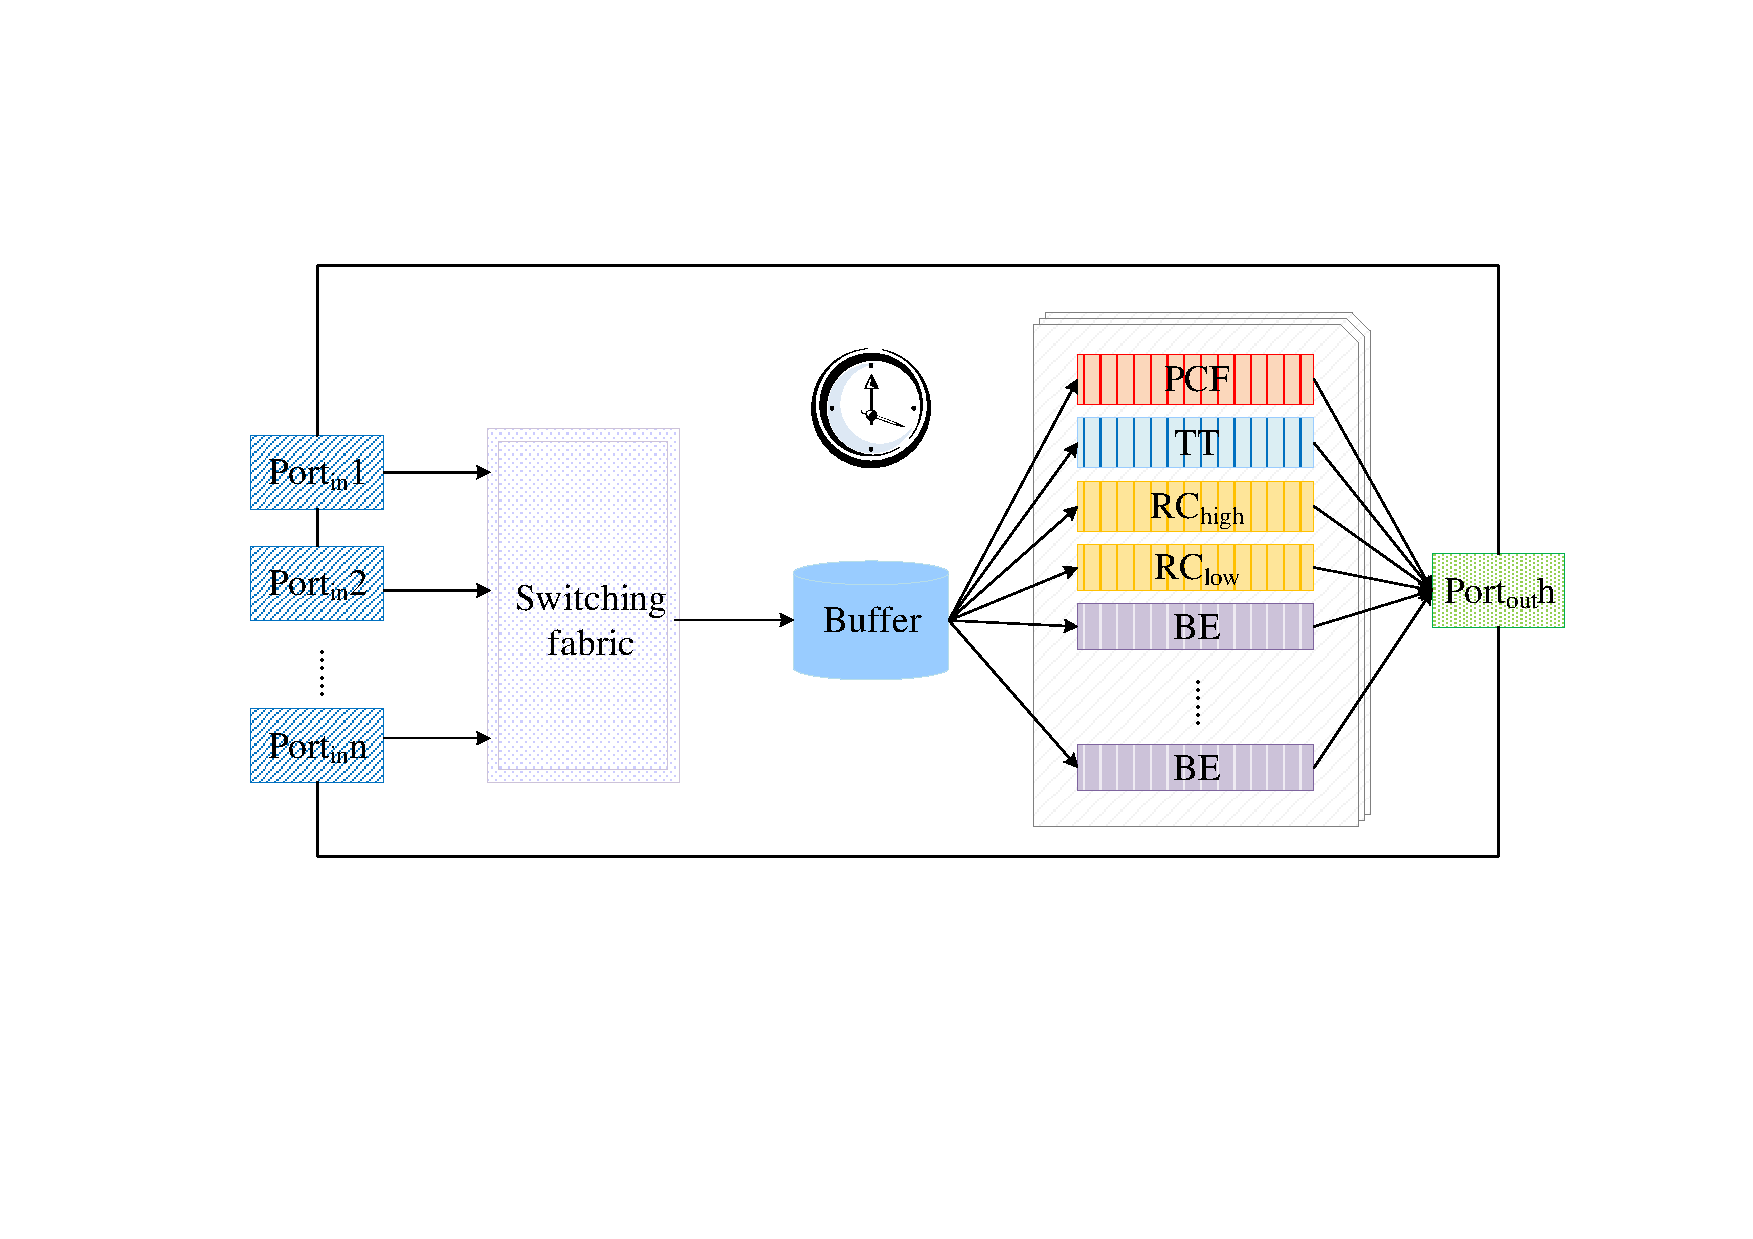
\includegraphics [scale=0.46] {figures/switch}
\caption{TTEthernet %Define, if appropriate.
	 switch architecture.}
\label{swi}
\end{figure}
The integrated transmission modes of TT and RC traffic are divided into three types: preemption, timely-block and shuffling \cite{kermia2017schedulability}, as shown in {Figure} \ref{inter}. Preemption indicates a RC frame can be preempted and relayed after the transmission of a TT frame. In timely-block mode, before a RC frame is transmitted, it needs to predict whether there is enough idle time between the next adjacent TT frame for its complete transmission. If not, the RC frame will be delayed for transmission. Shuffling is the mode in which TT frame will be delayed until the transmission for RC is finished.

\begin{figure}[H]
\centering
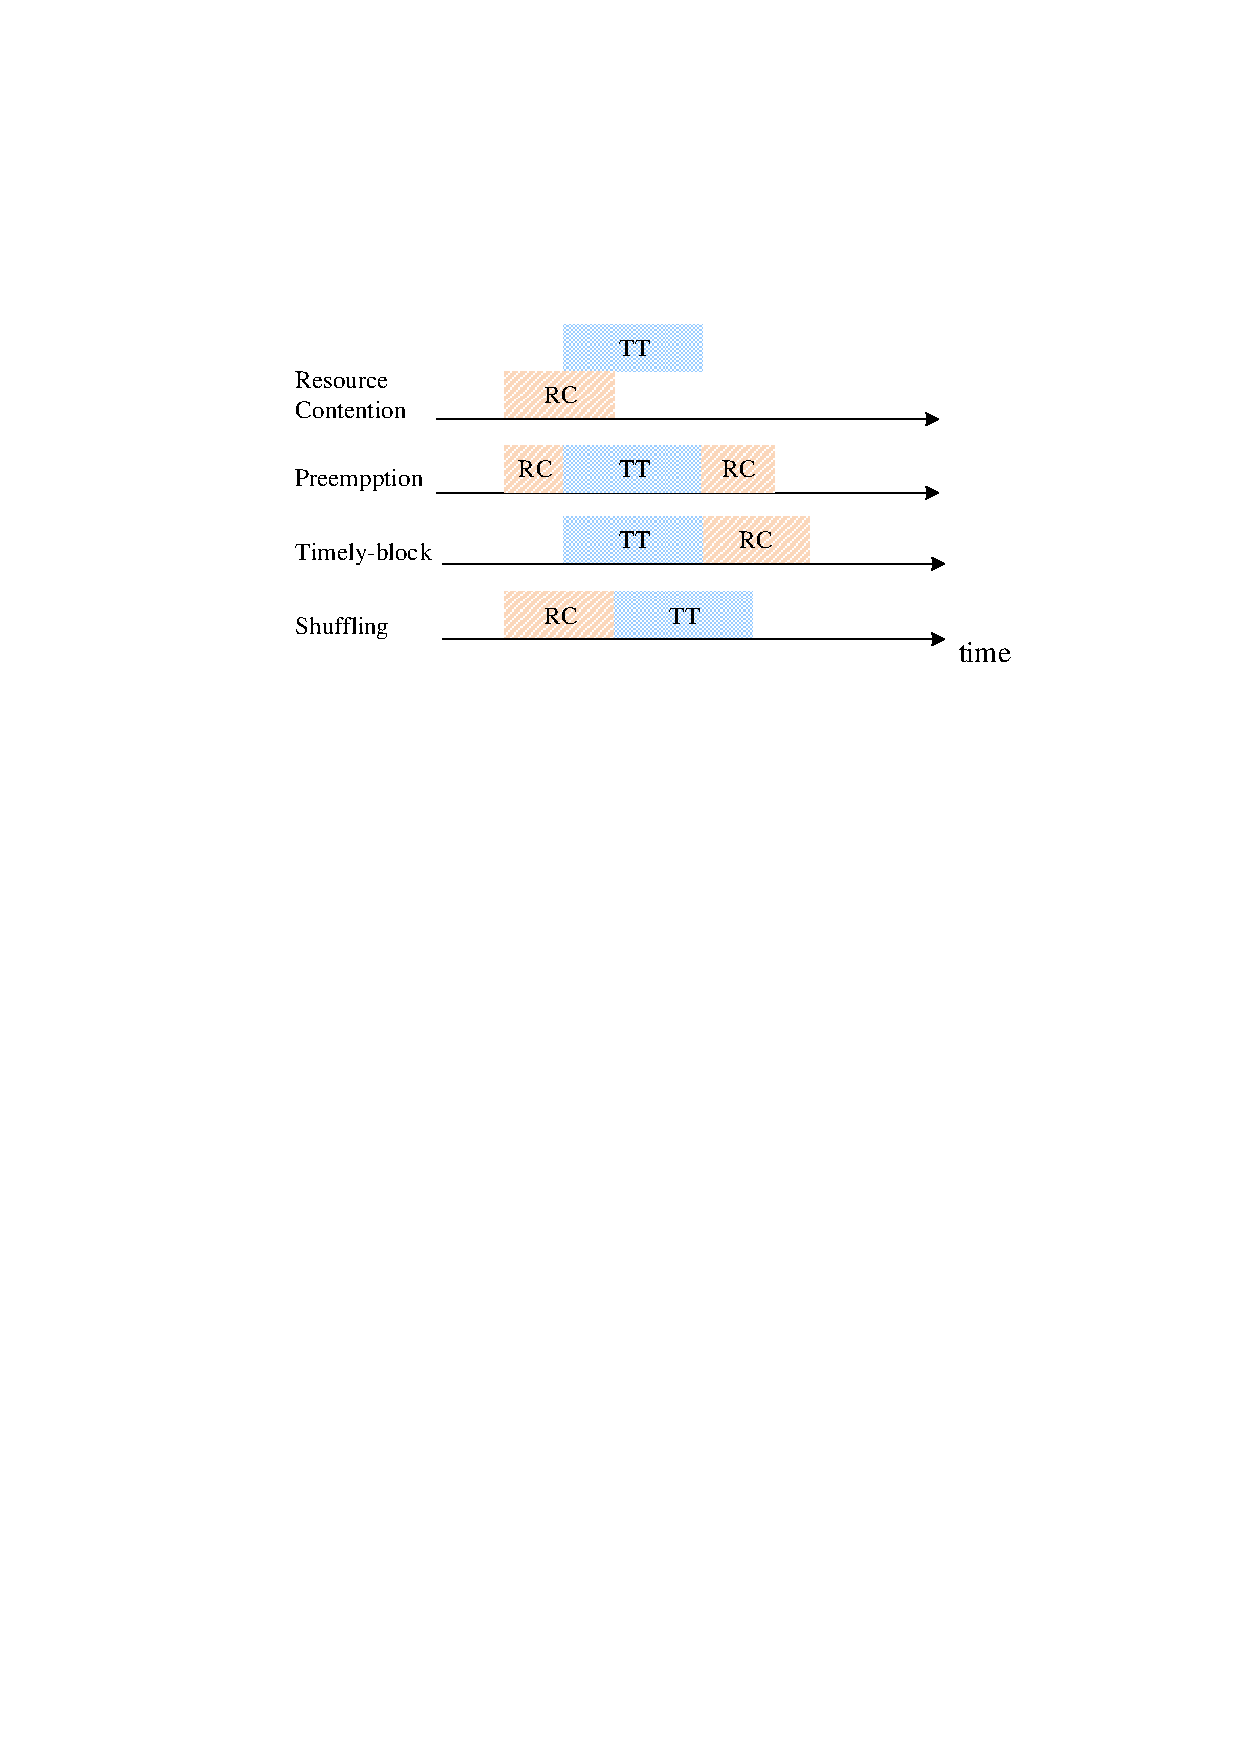
\includegraphics [scale=0.65] {figures/intergration}
\caption{Integration policies of time-triggered (TT) and rate-constrained (RC) traffic.}
\label{inter}
\end{figure}

\subsection{Real-Time Calculus}

Real-time calculus (RTC) is an extension of network calculus in real-time applications \cite{thiele2000real}. Network calculus \cite{le2001network} is a mathematical approach to modeling network behavior. RTC relies on the modeling of data flows and resources for processing components with curves called arrival curves and service curves. Arrival curves are functions of relative time to constrain the traffic that can occur in an interval of time. Service curves are used to count available resources. A component can be described with curves; then RTC gives exact delay bounds, backlog bounds and resource utilization for already-modeled components to evaluate network performance. The arrival curve and service curve are defined as follows.

\begin{myDef}[Arrival Curve]
 Given a time interval $[s,t)$, the cumulative function R(t) $\geq$ 0 represents the total number of data flows that has arrived in the network component up to time t. Further, assume that the amount of data flows arriving within any interval of time is bounded above by a function called the upper arrival curve, denoted by $\alpha^u$. Similarly, a lower bound on the number of data flows arriving is given by a lower arrival curve $\alpha^l$. $\alpha^l$ and $\alpha^u$ are related by the following inequality:
\begin{gather}
\begin{align}
	\alpha^l (t-s) \leq R(t) - R(s) \leq \alpha^u (t-s),\forall s<t %\label{con:1}
\end{align}
\end{gather}
where $\alpha^l$ (0) = $\alpha^u$ (0) = 0.
\end{myDef}

\begin{myDef}[Service Curve]
Given a time interval $[s,t)$, C(t) is a cumulative function that represents the available communication resources in the network component up to time t. Similarly to arrival curves, $\beta^u$ and $\beta^l$ denote upper and lower service curves of a resource respectively; the following inequality holds:
\begin{gather}
\begin{align}
	\beta^l (t-s) \leq C(t) - C(s) \leq \beta^u (t-s),\forall s<t %\label{con:2}
\end{align}
\end{gather}
where $\beta^l$ (0) = $\beta^u$ (0) = 0.
\end{myDef}

RTC is based on min-plus algebra and max-plus algebra. In these algebras, convolution and deconvolution are commonly used operations. These operations are defined as follows, where $inf$ means infimum (greatest lower bound) and $sup$ means supremum (least upper bound).

\begin{myDef}[Min-plus Algebra]
The min-plus convolution $\otimes$ and deconvolution $\oslash$ of $f$ and $g$ are defined as:

\begin{gather}
\begin{align}
 	&(f\otimes g)(t) = \inf_{0\leq s\leq t}\{f(t-s)+g(s)\}\\
 	&(f\oslash g)(t) = \sup_{s \ge 0}\{f(t+s)-g(s)\}
\end{align}
\end{gather}
\end{myDef}

The max-plus deconvolution is similar to the min-plus convolution.

\begin{myDef}[Max-plus Algebra]
The max-plus convolution $\overline{\otimes}$ and deconvolution $\overline{\oslash}$ of $f$ and $g$ are defined as:

\begin{gather}
\begin{align}
    &(f\overline{\otimes} g)(t) = \sup_{0 \leq u \leq t}\{f(t-u)+g(u)\}\\
 	&(f\overline{\oslash} g)(t) = \inf_{u \ge 0}\{f(t+u)-g(u)\}
\end{align}
\end{gather}
\end{myDef}

%%%%%%%%%%%%%%%%%%%%%%%%%%%%%%%%%%%%%%%%%%
\section{Performance Analysis Framework}
\label{per}

This section describes the construction of a performance analysis framework for TTEthernet. As~shown in {Figure} \ref{framework}, a data model, resource model and system model were devised and used to build the abstract model of the system required for the performance analysis of TTEthernet. The data model is mainly described by the arrival curve under the traffic configuration. The resource model is represented by the service curve under different scheduling strategies. The system model was built based on component model and system architecture. For already-modeled abstract model, RTC was applied to analyze network performance and get analysis results.

\begin{figure}[H]
\centering
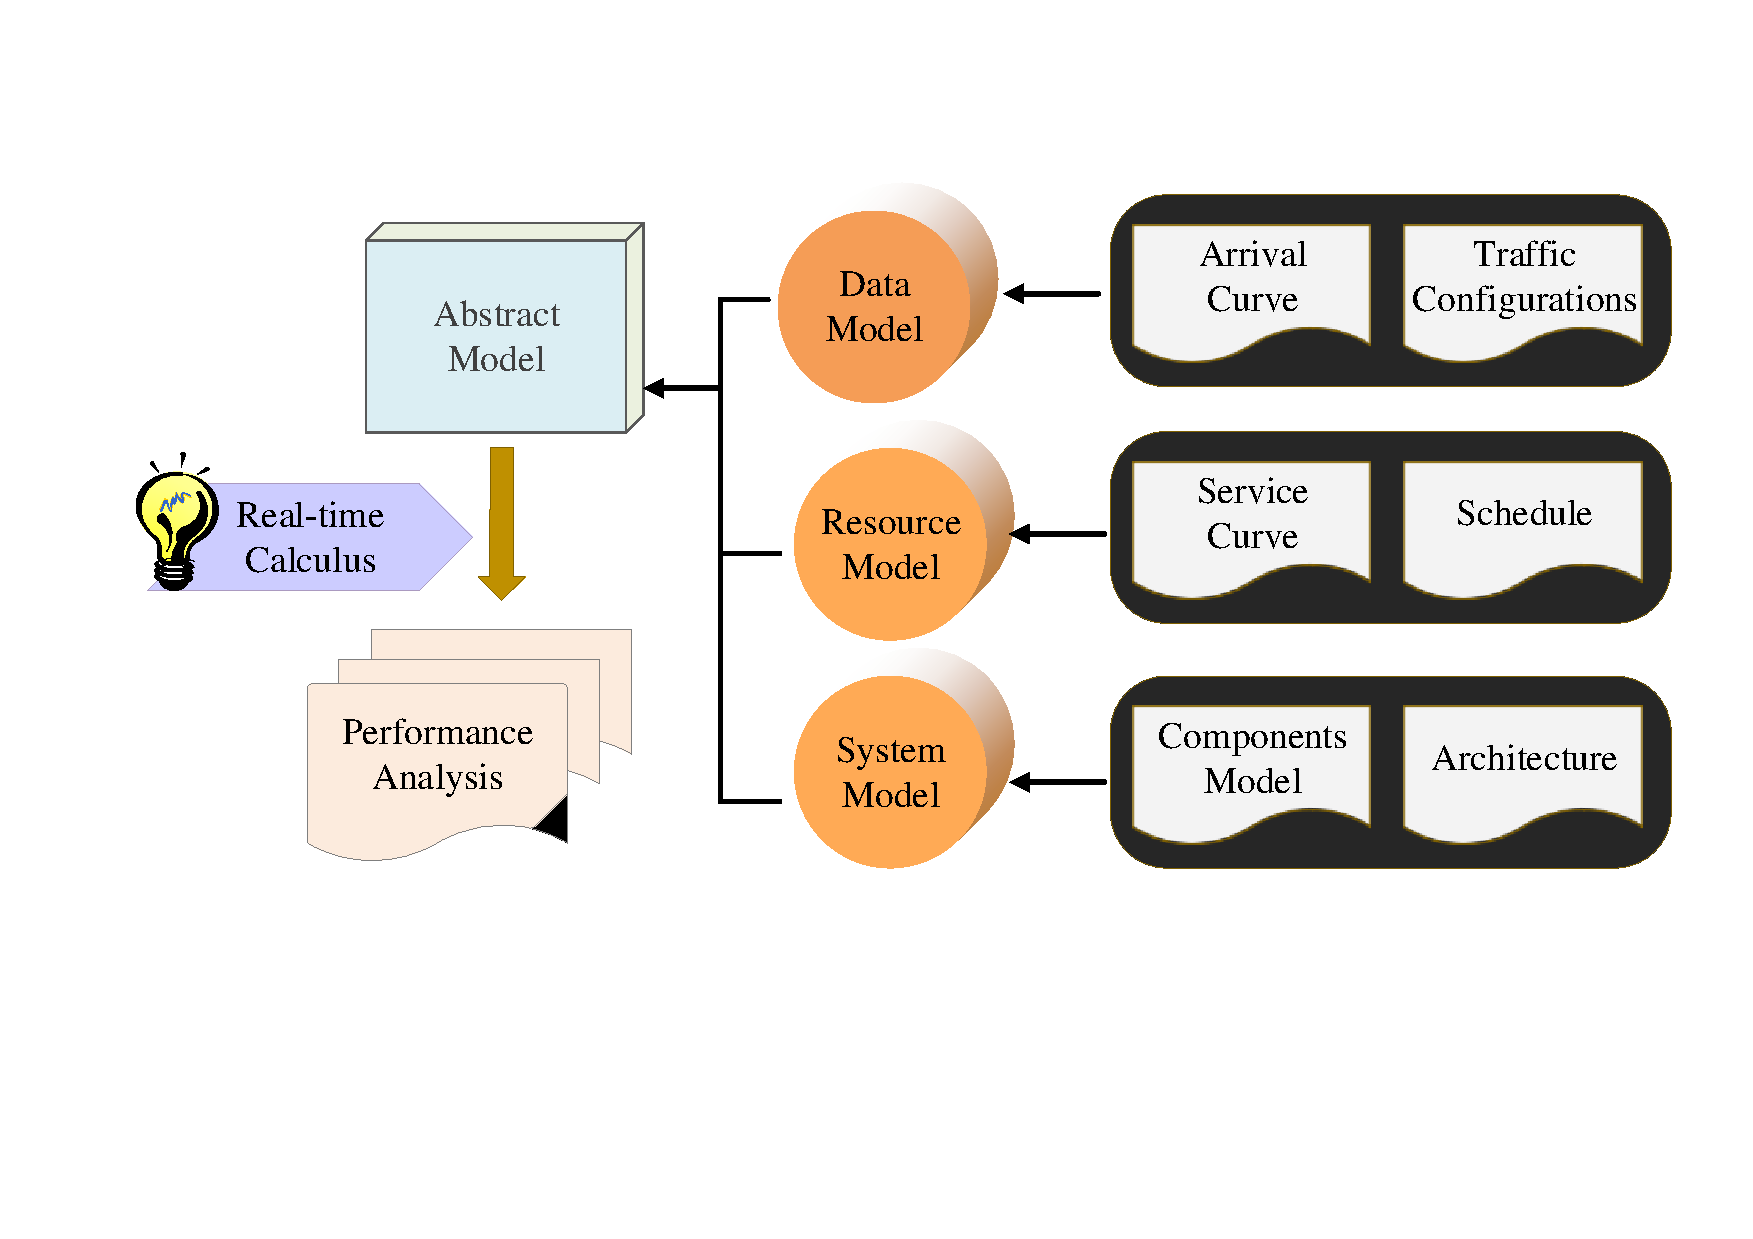
\includegraphics [scale=0.4] {figures/framework}
\caption{Performance analysis framework of TTEthernet.}
\label{framework}
\end{figure}


\subsection{Data Model}

The data model is described by the arrival curve, which defines lower and upper bounds on the amount of data flows that can occur in a window of time \cite{le1998application}. Since TT frames can only be served in reserved time slots, the arrival curve of TT flow can be represented by a staircase function. The arrival curve of a single TT flow is given by Equation (7).

\begin{gather}
\begin{align}
	\alpha_{TT}(t)=\begin{cases}
	l_{TT}\cdot \left \lceil \frac{t+\triangle}{P_{TT}} \right \rceil,
	\qquad & t>0 \\
	0, \qquad & t\le0
\end{cases}
\end{align}
\end{gather}
where $P_{TT}$ is the periodic of TT flow, $l_{TT}$ represents the frame length and $\triangle$ is the delay variation.

However, multiple TT flows are often transmitted on the same port. Therefore, an aggregate arrival curve of TT flows needs to be processed. As shown in {Figure} \ref{lcm}, it is assumed that there are three types of TT flows which are transmitted at one output port, with their periods $P_{TT_1}$ = 2 ms,\  $P_{TT_2}$ = 3 ms and\  $P_{TT_3}$ = 6 ms. Since all TT flows are scheduled periodically, the aggregate TT flows will be scheduled based on the least common multiple period ($P_{LCM}$) of these three TT flows. As shown in {Figure} \ref{lcm}, the $P_{LCM}$ of these three flows is 6 ms.

\begin{figure}[H]
\centering
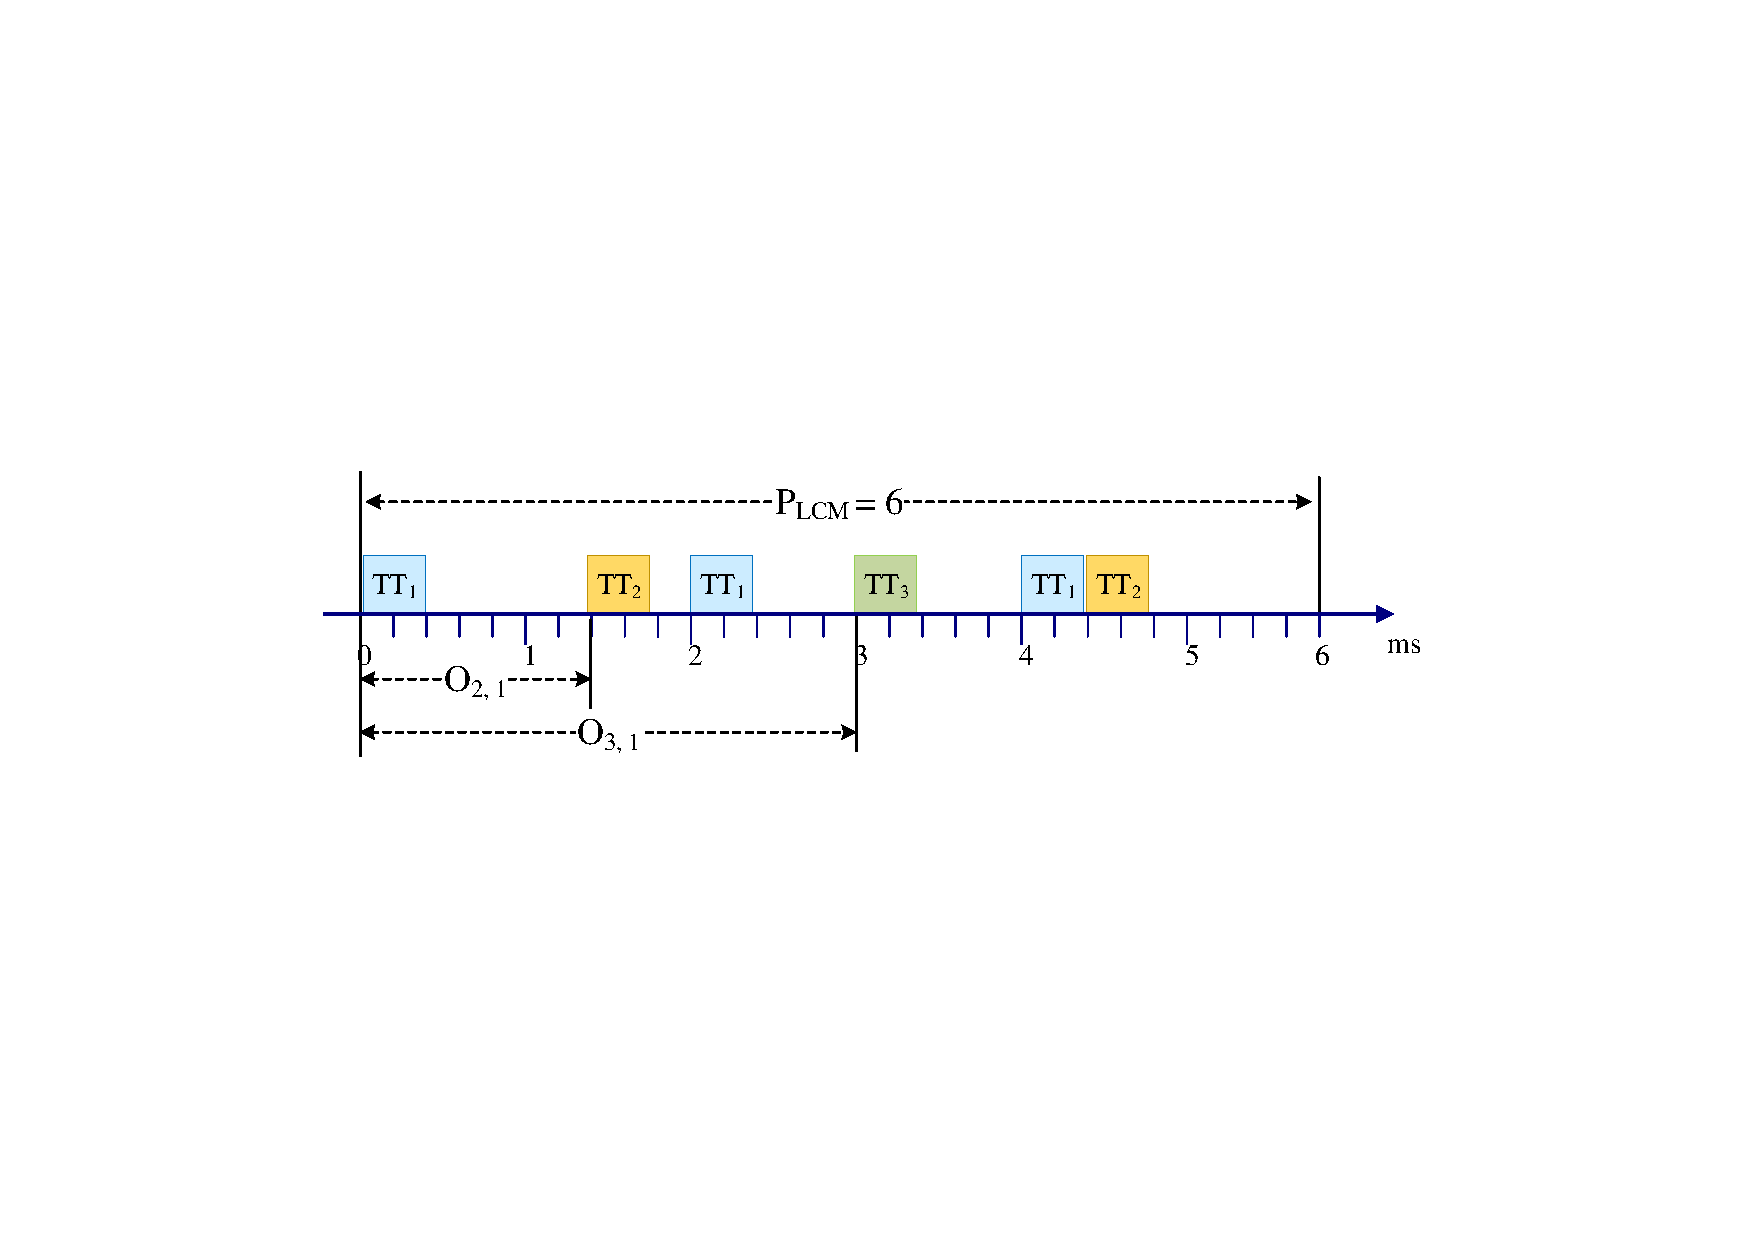
\includegraphics[scale=0.52] {figures/LCM}
\caption{Period of aggregated TT flows.}
\label{lcm}
\end{figure}

To obtain the aggregated arrival curves of all TT flows, one TT flow is used as a reference to analyze the arrival curves of other flows. Thereafter, the arrival curves of all TT flows are accumulated to obtain the aggregated arrival curve of the reference one \cite{moy2010arrival}. Assuming that the flow $TT_i$ is used as a reference, the upper aggregated arrival curve $\alpha^{i,u}_{TT}(t)$ and the lower aggregated arrival curve $\alpha^{i,l}_{TT}(t)$ about $TT_i$ are given by Equations (8) and (9).

\begin{gather}
\begin{align}
	\alpha^{i,u}_{TT}(t) &= \sum_{k=1}^{N_{TT}} \alpha_{TT_k}^u(t-O_{k,i})\\
%\end{align}
%\end{gather}
%\begin{gather}
%\begin{align}
	\alpha^{i,l}_{TT}(t) &= \sum_{k=1}^{N_{TT}} \alpha_{TT_k}^l(t-O_{k,i})
\end{align}
\end{gather}
where $O_{k,i}$ is the relative offset which defines the interval between the first frame of the reference flow $TT_i$ and the first frame of the flow $TT_k$. $N_{TT}$ refers to the number of TT traffic.

$\alpha^{i,u}_{TT}(t)$ and $\alpha^{i,l}_{TT}(t)$ can be calculated by the upper arrival curve and the lower arrival curve of a single TT flow given by
\begin{gather}
\begin{align}
	\alpha_{TT_k}^u(t)&=\begin{cases}
 	\min \{ {l_{TT_k}\cdot \left \lceil \frac{t+j}{P_{TT_k}} \right \rceil} , \lceil \frac{t}{d} \rceil \},
	\qquad & t>0 \\
	0, \qquad & t\le0
\end{cases}\\
%\end{align}
%\end{gather}
%\begin{gather}
%\begin{align}
	\alpha_{TT_k}^l(t)&=\begin{cases}
	l_{TT_k}\cdot \left \lceil \frac{t-j}{P_{TT_k}} \right \rceil,
	\qquad ~~~~~~~~~~& t>0 \\
	0, \qquad ~~~~~~~& t\le0
\end{cases}
\end{align}
\end{gather}
where $j$ is the jitter of TT flows, $d$ is the minimum interval distance of traffic and $d$ is much smaller than~$P_{TT_{k}}$.

There are three TT flows in {Figure} \ref{lcm}, and we can get three different aggregate arrival curves with these TT flows as references, as shown in {Figure} \ref{arr}. The blue and gray dotted lines indicate upper arrival curves and lower arrival curves for each of these flows. Finally, the worst-case upper aggregate arrival curve $\alpha_{TT}^u(t)$ and the lower aggregate arrival curve $\alpha_{TT}^l(t)$ are represented by red and green solid lines, respectively. Their formula is given in Equations (12) and (13).
\begin{gather}
\begin{align}
	\alpha_{TT}^u(t) &= \max_{1 \leq i \leq {N_{TT}}} \{  \alpha_{TT}^{i,u}(t) \}\\
%\end{align}
%\end{gather}
%\begin{gather}
%\begin{align}
	\alpha_{TT}^l(t) &= \min_{1 \leq i \leq {N_{TT}}} \{  \alpha_{TT}^{i,l}(t) \}
\end{align}
\end{gather}

\begin{figure}[H]
\centering
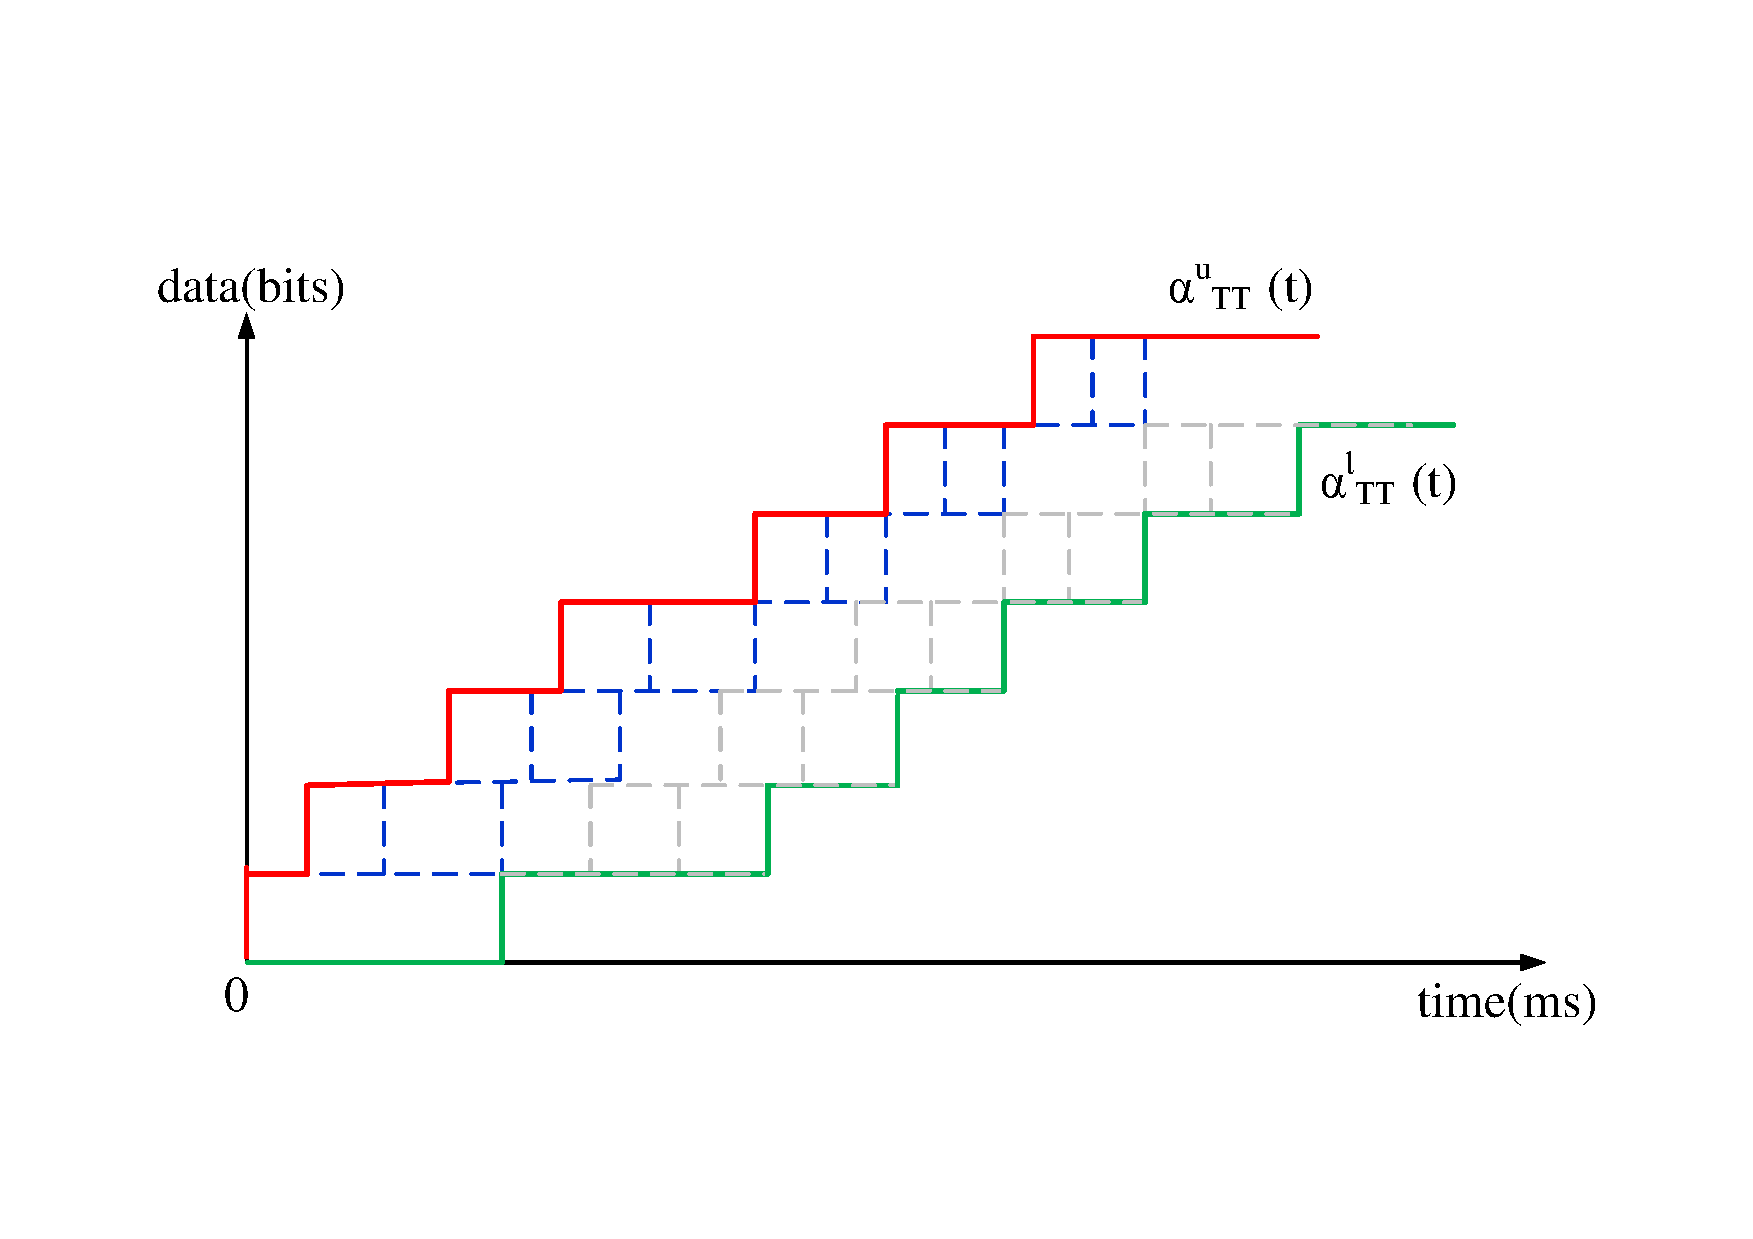
\includegraphics[scale=0.35] {figures/arrival}
\caption{Aggregate arrival curve of TT flows.}
\label{arr}
\end{figure}
\subsection{Resource Model}

The resource model is described by a service curve, which represents the amount of data that a component can process. Here we suppose that the scheduling strategy is known, to analyze the data processing ability of nodes under this scheduling strategy.

\textls[-5]{In a time-triggered system, the schedule defines the "receiving point" (the expected time of transmission)} of TT traffic. Due to clock drifts and jitter, the receiving point is not exactly known and thus acceptance windows are given \cite{perathoner2007influence}. The acceptance windows is a predefined duration interval around the expected "receiving point." If a transmission occurs within the defined acceptance window, the transmission is "scheduled"; otherwise it is "unscheduled" and such unscheduled transmission is considered to be invalid. The size of acceptance window for TT flow is predefined, but under the influence of clock synchronization and traffic integration strategies, the actual open window is smaller than a predetermined window.

As is shown in {Figure} \ref{inf}, we give an example to illustrate the influence of clock synchronization and traffic integration strategy on the acceptance windows of TT flows. In this example, it is assumed that $P_{LCM}$ of TT flow is 6ms and consists of three TT flows. $W_{TT}$ represents a predefined acceptance window of TT flow, and $W^*_{TT}$ represents an actual open acceptance window after considering the effects of clock synchronization and traffic integration strategies. Suppose that the i-th time slot of TT transmission is used as the reference point for next calculation. $O^{j,i}_{TT}$ represents the time interval between the i-th open window and the j-th open window. $I^i_{TT}$ represents the longest waiting time before the i-th open window.

\begin{figure}[H]
\centering
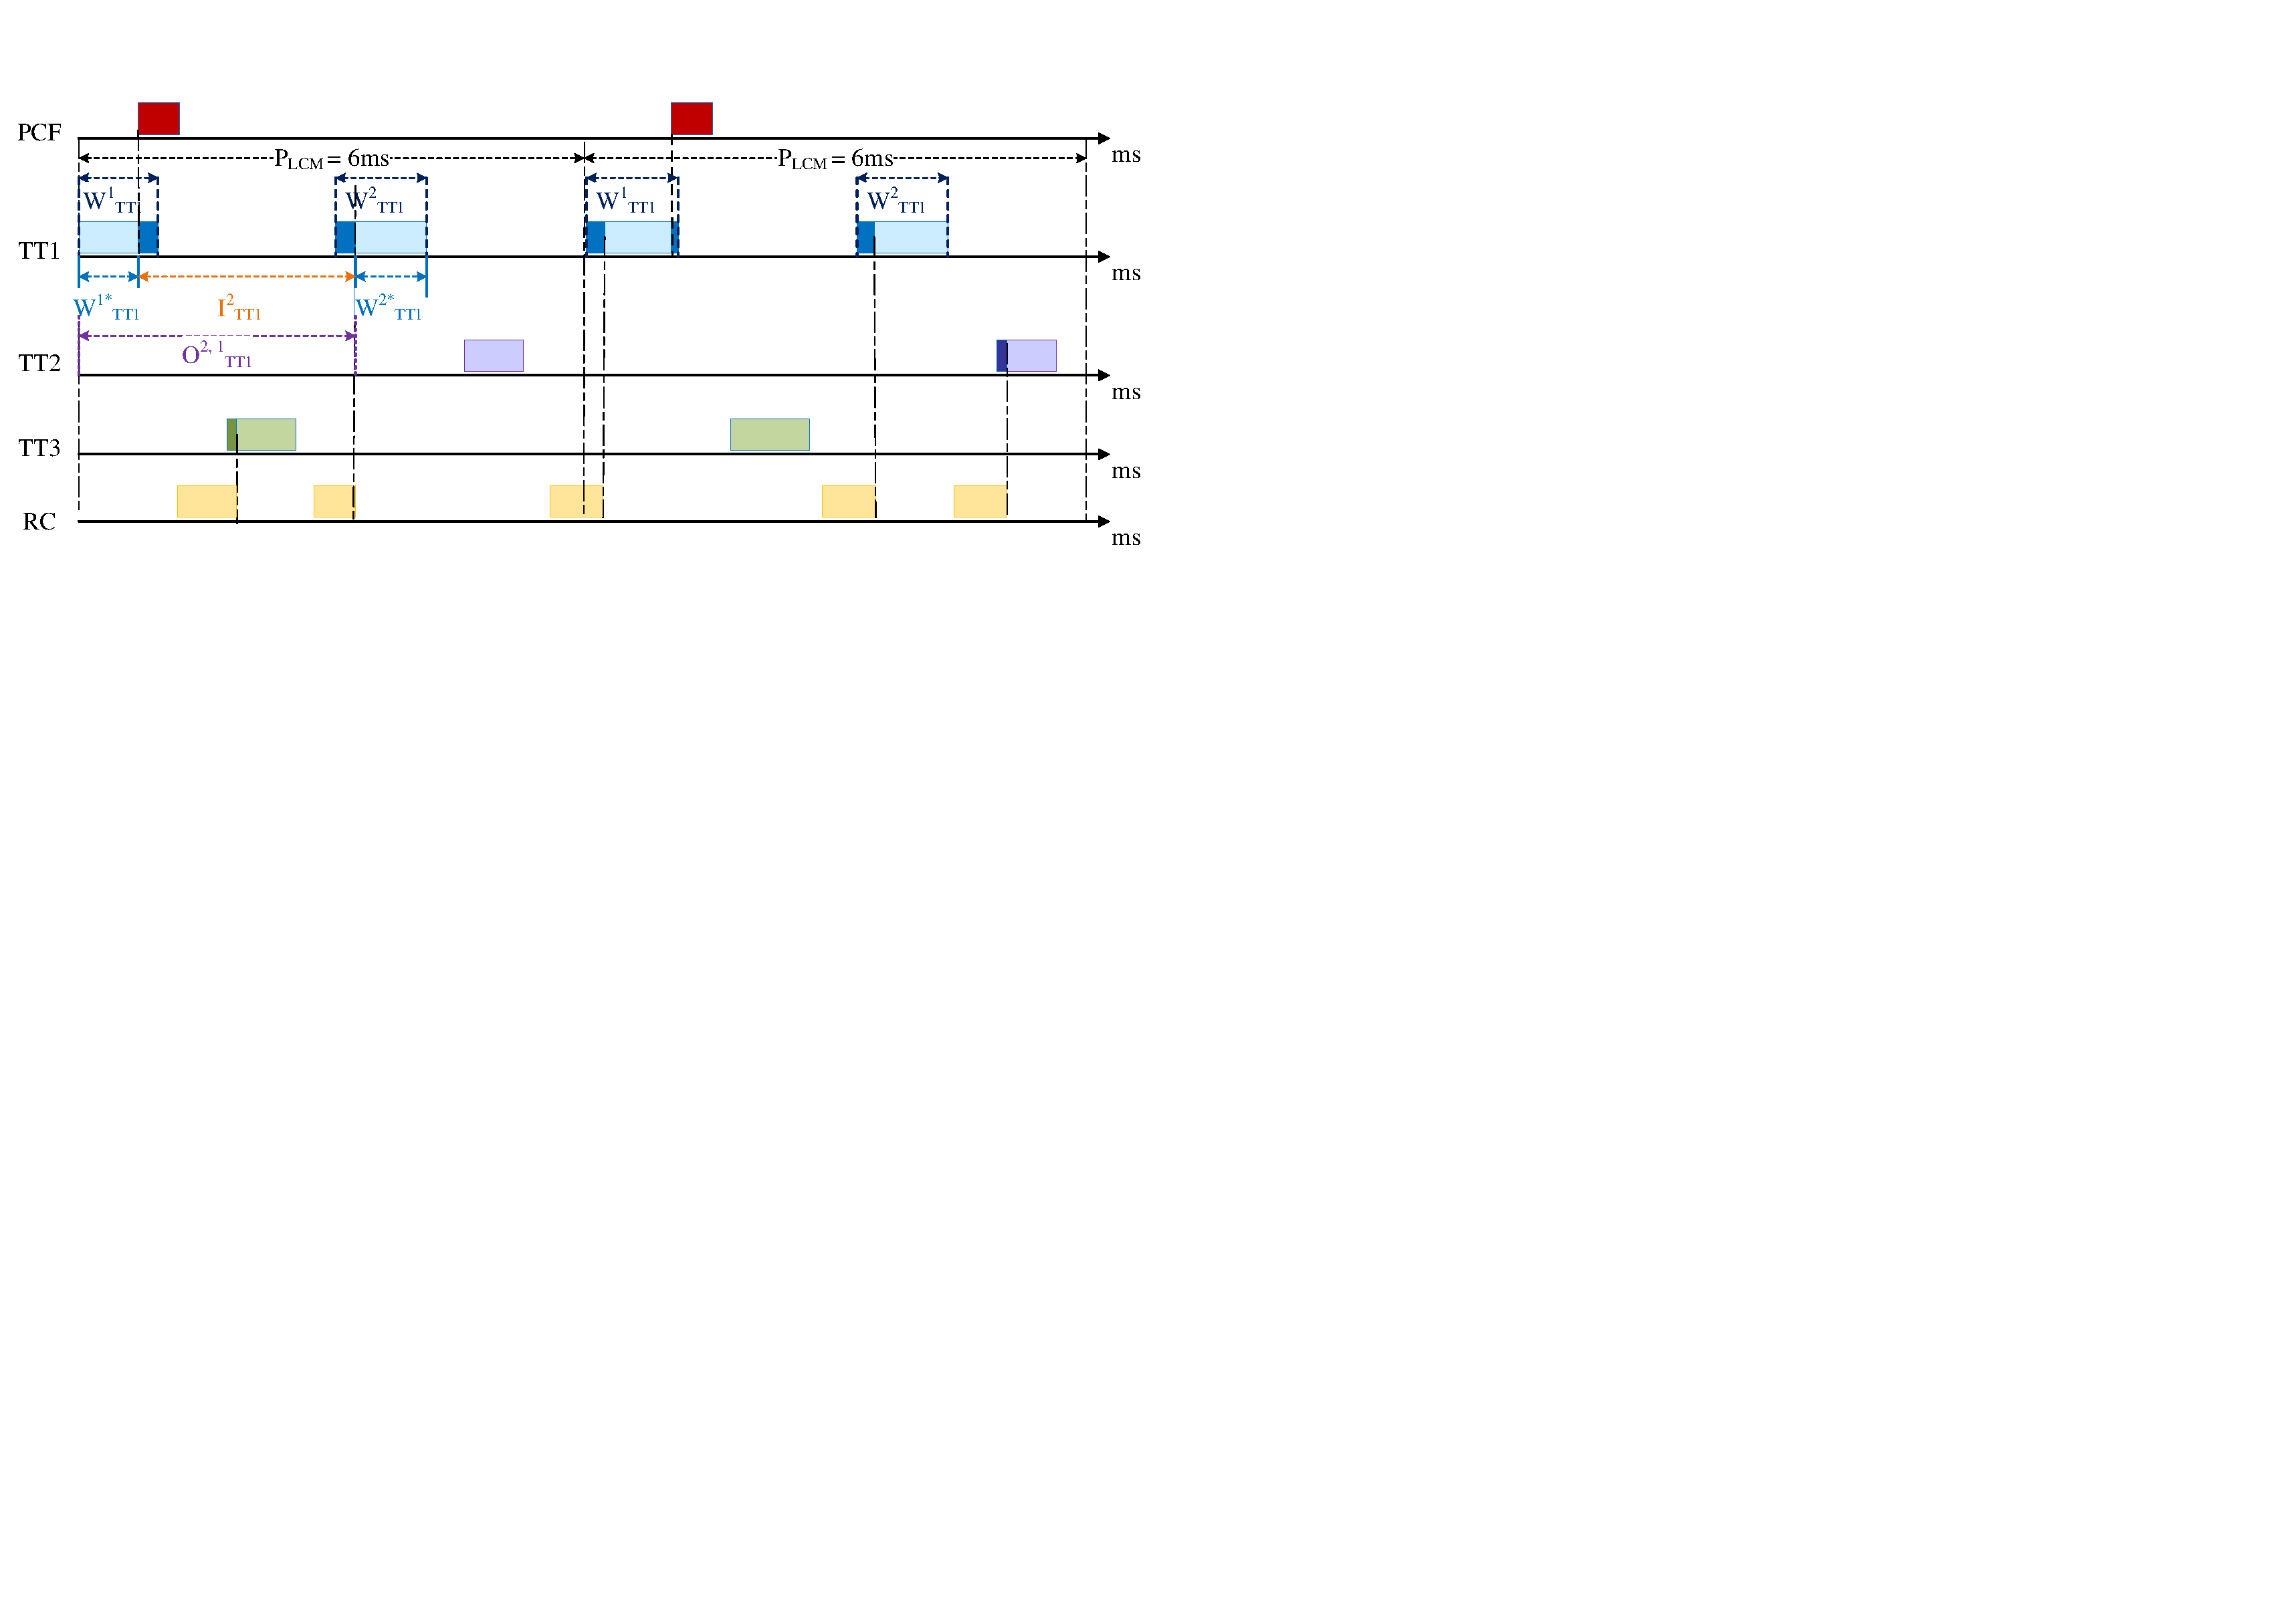
\includegraphics[scale=0.44]{figures/pri_influ}
\caption{Acceptance windows for TT.}
\label{inf}
\end{figure}

It is vital to ensure clock synchronization for TT frame transmission. If clock synchronization cannot be maintained, the transmission will be congested and blocked, thereby impacting real-time of critical traffic.
TTEthernet defines dedicated synchronization messages as the PCFs, whose priority should be higher than that of TT frames, so that the transmission of PCFs will have an impact on acceptance windows of TT frames. There are three types of PCF: cold-start (CS) frame, cold-start acknowledge (CA) frame and~integration (IN) frame. The first two are executed to reach  an initial synchronization of the local clocks in  the system. The latter is executed during normal operation mode to keep the local clocks synchronized to each other and used for components to join an already synchronized system. {Figure} \ref{inf} shows the effect of IN frames on the TT acceptance window. The time slot of the PCFs indicates that clock synchronization will be performed during this period, so PCFs will preempt TT traffic during this period, thereby affecting the size of the TT acceptance window. As shown in {Figure} \ref{inf}, the expected acceptance window $W^1_{TT1}$ in first $P_{LCM}$ will be reduced under the influence of PCFs. After being preempted by PCFs, the actual open window of TT1 becomes $W^{1*}_{TT1}$. Suppose $t^{o,i}_{TT_{pcf}}$ and $t^{c,i}_{TT_{pcf}}$  represent the opening and closing times of the TT acceptance window under the influence of PCFs respectively. $t^{o,i}_{TT_{pcf}}$ and $t^{c,i}_{TT_{pcf}}$ are calculated by Equations (14) and (15).
\begin{gather}
\begin{align}
	t^{o,i}_{TT_{pcf}} &= t^{o,i}_{TT} + d^{o,i}_{TT_{pcf}}\\
%\end{align}
%\end{gather}
%\begin{gather}
%\begin{align}
	t^{c,i}_{TT_{pcf}} &= t^{c,i}_{TT} - d^{c,i}_{TT_{pcf}}
\end{align}
\end{gather}
where $t^{o,i}_{TT}$ and $t^{c,i}_{TT}$ represent the opening and closing times of the expected TT window respectively. $d^{o,i}_{TT_{pcf}}$ and $d^{c,i}_{TT_{pcf}}$ are open delay and closed delay of TT acceptance window under the influence of PCFs respectively and given by
\begin{gather}
\begin{align}
	d^{o,i}_{TT_{pcf}}&=\begin{cases}
	\min \{ \frac{l^{max}_{pcf}}C, t^{c,i}_{PCF} - t^{o,i}_{TT}\},
	\qquad &  t^{o,i}_{TT} < t^{c,i}_{PCF}\\
	0, \qquad &  t^{o,i}_{TT} \geq t^{c,i}_{PCF}
\end{cases}\\
%\end{align}
%\end{gather}
%\begin{gather}
%\begin{align}
	d^{c,i}_{TT_{pcf}}&=\begin{cases}
	t^{c,i}_{TT} - t^{o,i}_{PCF} ,
    \qquad ~~~~~~~~~~~&  t^{c,i}_{TT} > t^{o,i}_{PCF}\\
	0, \qquad ~~~~~~~~&  t^{c,i}_{TT} \leq t^{o,i}_{PCF}
\end{cases}
\end{align}
\end{gather}
where $l^{max}_{pcf}$ is the maximum length of PCFs and C is the physical link rate. Similarly, $t^{o,i}_{PCF}$ and $t^{c,i}_{PCF}$ are the opening and closing times of PCF transmission.

\textls[-5]{There exists competition in TTEthernet when a RC frame is already for transmission while encountering} a TT acceptance window.~Three integration strategies of TT and RC, i.e.,  preemption, timely-block and shuffling, are illustrated in {Figure} \ref{inter}. In preemption and timely-block strategies, RC frame will not cause the delay for TT frame's transmission. Thus, a TT acceptance window has no effect under these two strategies. Under the shuffling integration strategy, if a TT frame is scheduled while an RC frame is already being transmitted, then the TT frame will be delayed until the transmission of RC is finished. Therefore, the~transmission of RC frame has an influence on acceptance window of  TT in a shuffling strategy. As shown in {Figure} \ref{inf}, for the acceptance window $W^2_{TT1}$ in the first $P_{LCM}$, the actual acceptance window is $W^{2*}_{TT1}$ under the influence of a shuffling integration strategy. Suppose $t^{o,i}_{TT_{rc}}$ represents the opening time of TT acceptance window affected by integration strategies. $t^{o,i}_{TT_{rc}}$ is given by Equation (18).
\begin{gather}
\begin{align}
&	t^{o,i}_{TT_{rc}} = t^{o,i}_{TT} + d^{o,i}_{TT_{rc}}
\end{align}
\end{gather}
where $d^{o,i}_{TT_{rc}}$ indicates the delay of TT acceptance window under the influence of integration strategy. Note~that $d^{o,i}_{TT_{rc}}$ is caused by the shuffling integration strategy and expressed as follows:
\begin{gather}
\begin{align}
	d^{o,i}_{TT_{rc}}=\begin{cases}
	\min \{ \frac{l^{max}_{RC}}C, t^{c,i}_{RC}-t^{o,i}_{TT}\},
	\qquad &  t^{o,i}_{TT} < t^{c,i}_{RC}\\
	0, \qquad &  t^{o,i}_{TT} \geq t^{c,i}_{RC}
\end{cases}
\end{align}
\end{gather}
where $l^{max}_{RC}$ represents the maximum length of the RC frames and $t^{c,i}_{RC}$ is the end time of RC transmission.

Considering the influence of clock synchronization and integration strategy, the start time $t^{s,i}_{TT}$ and end time $t^{e,i}_{TT}$ of actual acceptance window for TT are as follows:
\begin{gather}
\begin{align}
	t^{s,i}_{TT} &= \max \{ t^{o,i}_{TT}, t^{o,i}_{TT_{pcf}}, t^{o,i}_{TT_{rc}} \}\\
%\end{align}
%\end{gather}
%\begin{gather}
%\begin{align}
	t^{e,i}_{TT} &= \min \{ t^{c,i}_{TT}, t^{c,i}_{TT_{pcf}} \}
\end{align}
\end{gather}

Therefore, an actual acceptance window for TT is
\begin{gather}
\begin{align}
	W^{i*}_{TT}=\begin{cases}
	\max \{t^{e,i}_{TT}-t^{s,i}_{TT}, \frac{l^{min}_{TT}}C \},
	\qquad & t^{s,i}_{TT} < t^{e,i}_{TT} \\
	0, \qquad  & t^{s,i}_{TT} \geq t^{e,i}_{TT}
\end{cases}
\end{align}
\end{gather}

Assuming the i-th acceptance window is used as a baseline, the upper service curve $\beta^{i,u}_{TT}$ and the lower service curve $\beta^{i,l}_{TT}$ for TT traffic in a $P_{LCM}$ are given by
\begin{gather}
\begin{align}
	\beta^{i,u}_{TT}(t) &= \sum_{j=i}^{i+N_{TT}-1} \beta^{j,i,u}_{TT}(t)\\
%\end{align}
%\end{gather}
%\begin{gather}
%\begin{align}
	\beta^{i,l}_{TT}(t) &= \sum_{j=i}^{i+N_{TT}-1} \beta^{j,i,l}_{TT}(t)
\end{align}
\end{gather}
where $N_{TT}$ is the amount of TT traffic. $\beta^{j,i,u}_{TT}$ and $\beta^{j,i,l}_{TT}$ are as follows:

\begin{gather}
\begin{align}
	\beta^{j,i,u}_{TT} &= \beta_{P_{LCM},W^{j*}_{TT}}(t+P_{LCM}-W^{j*}_{TT}-O^{j,i}_{TT})\\
%\end{align}
%\end{gather}
%\begin{gather}
%\begin{align}
	\beta^{j,i,l}_{TT} &= \beta_{P_{LCM},W^{j*}_{TT}}(t+P_{LCM}-W^{j*}_{TT}-I^i_{TT}-O^{j,i}_{TT})
\end{align}
\end{gather}

$O^{j,i}_{TT}$ is the time interval between the j-th open window and the i-th open window and can be obtained by the following formula:
\begin{gather}
\begin{align}
&	O^{j,i}_{TT} = (j-i) \cdot P_{TT} + O^{j*}_{TT} - O^{i*}_{TT}
\end{align}
\end{gather}
where
\begin{gather}
\begin{align}
&	O^{i*}_{TT} = t^{s,i}_{TT} - t^{o,i}_{TT}
\end{align}
\end{gather}

 $I^i_{TT}$ represents the longest waiting time before the i-th open window.
\begin{gather}
\begin{align}
&	I^{i}_{TT} = t^{s,i}_{TT} - t^{e,i-1}_{TT}
\end{align}
\end{gather}

The service curve $\beta_{P_{LCM},W^{j*}_{TT}}(t)$ is calculated by
\begin{gather}
\begin{aligned}
 	\beta_{T,L}(t) = C \cdot max(\left \lfloor \frac{t}{L} \right \rfloor L,t-\left \lceil \frac{t}{L} \right \rceil(T-L))
\end{aligned}
\end{gather}

By considering the different baselines, the final upper service curve of $\beta^u_{TT}(t)$ and the final lower service curve
$\beta^l_{TT}(t)$ of TT flows are given by Equations (31) and (32).
\begin{gather}
\begin{align}
	\beta^u_{TT}(t) &= \max_{1\leq i\leq N_{TT}} \{ \beta^{i,u}_{TT}(t)\}  \\
%\end{align}
%\end{gather}
%\begin{gather}
%\begin{align}
	\beta^l_{TT}(t) &= \min_{1\leq i\leq N_{TT}} \{ \beta^{i,l}_{TT}(t) \}
\end{align}
\end{gather}

{Figure} \ref{ser} shows the worst-case service curve of $TT1$ traffic for the example above.

\begin{figure}[H]
\centering
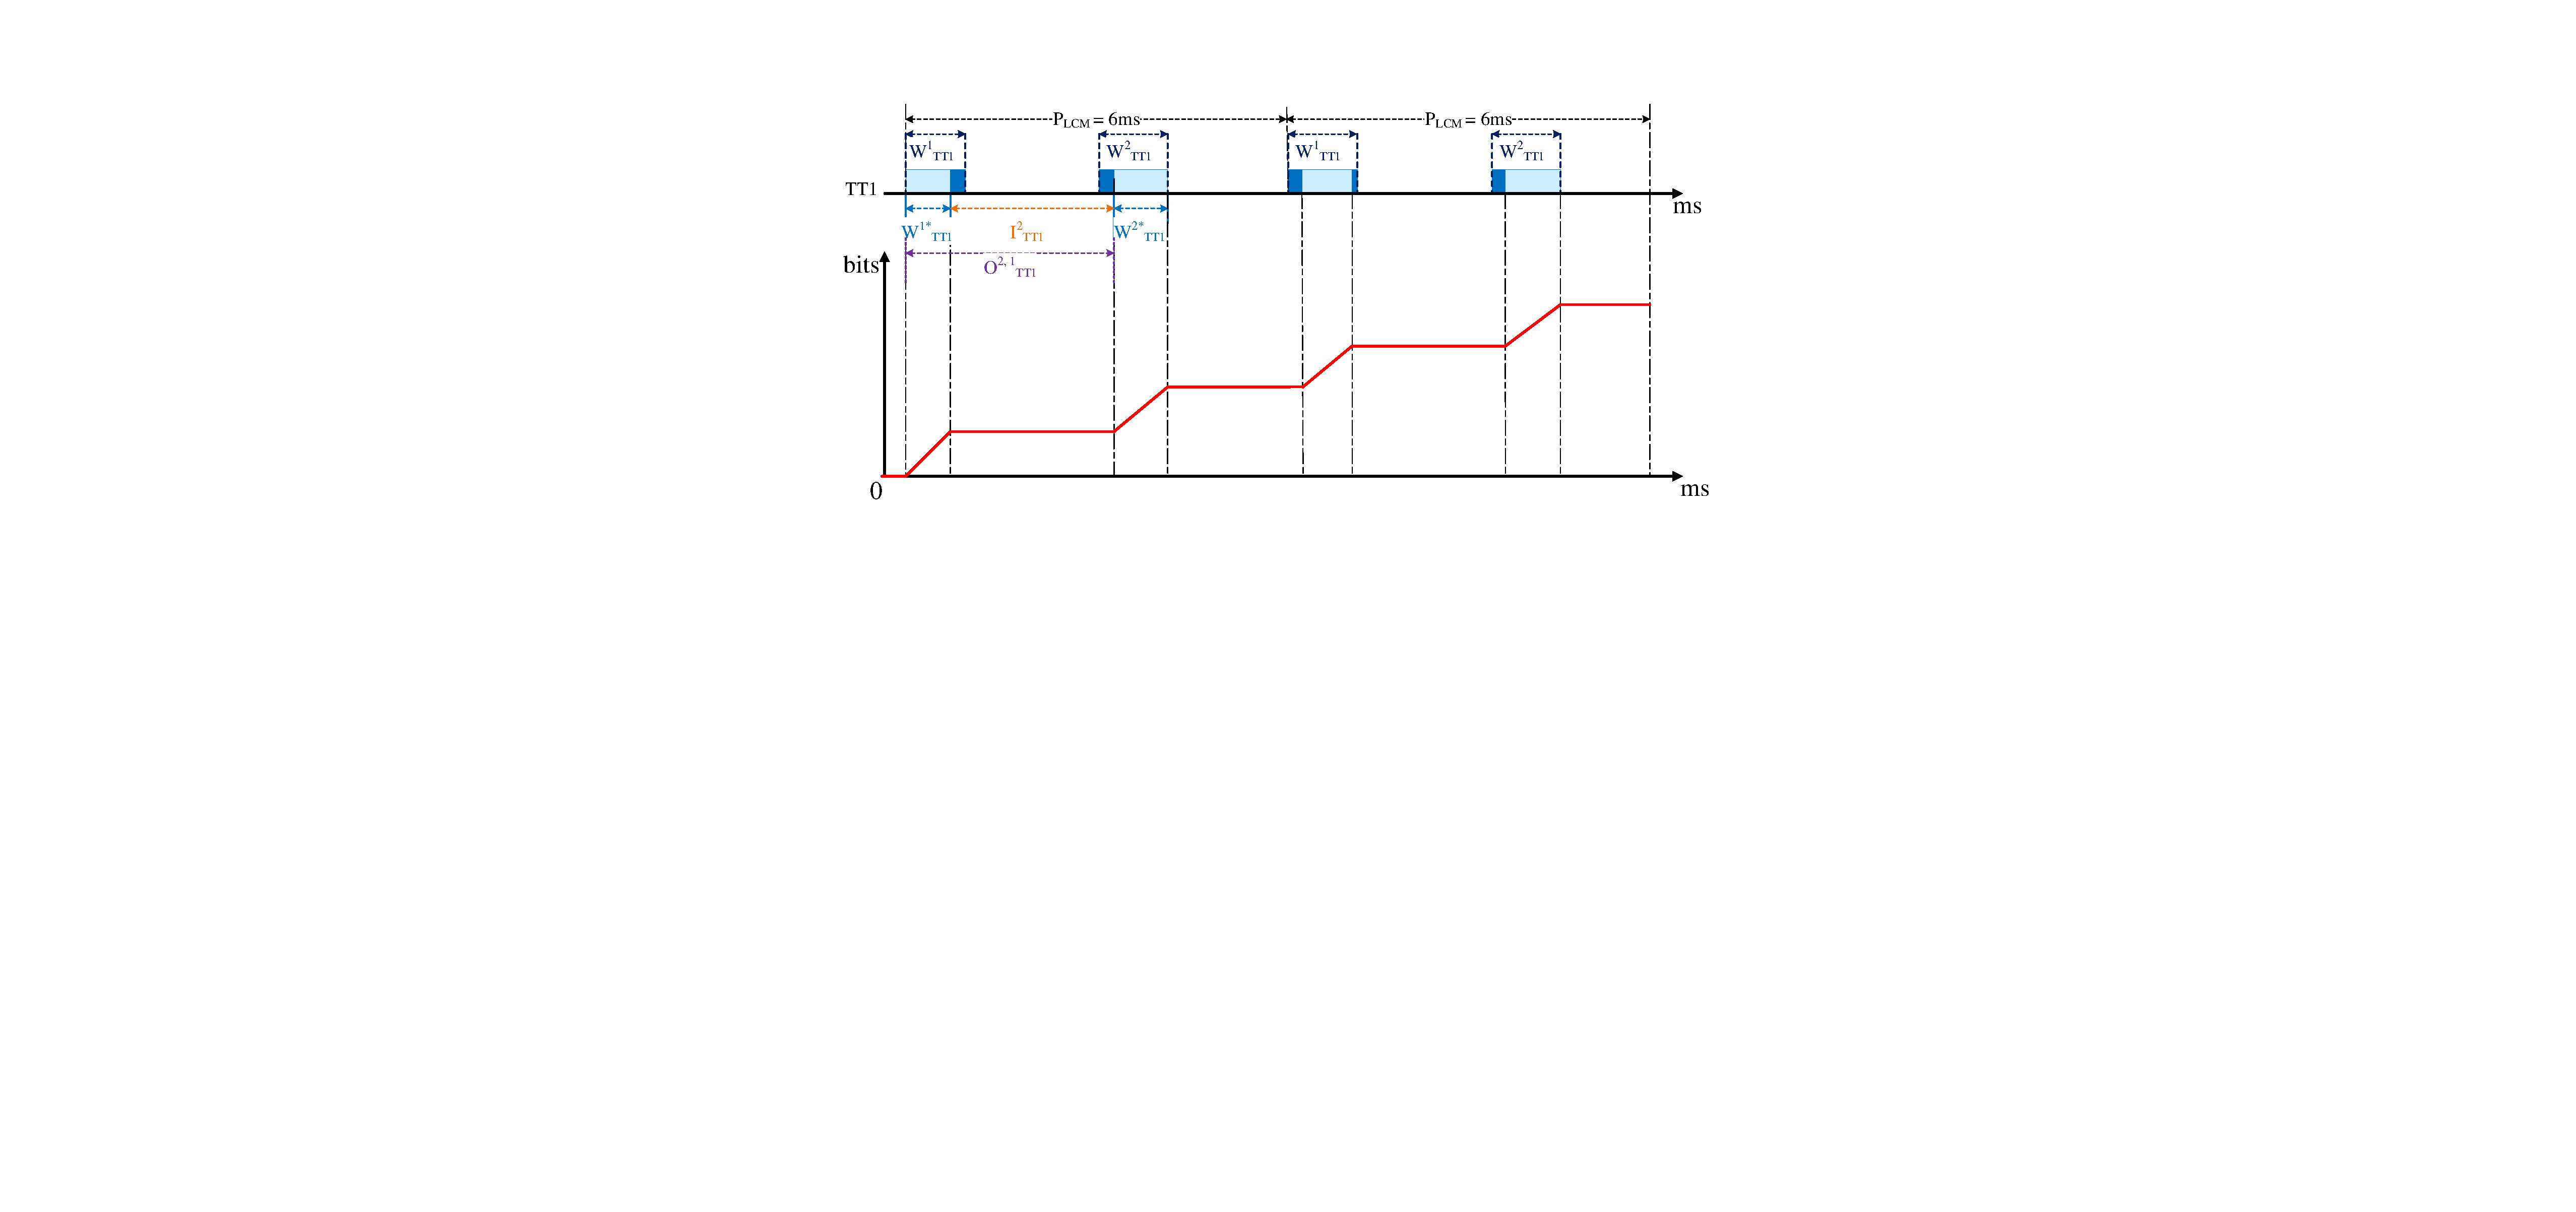
\includegraphics[scale=0.4]{figures/service}
\caption{Worst-case service curve of TT1.}
\label{ser}
\end{figure}

\subsection{Abstract Model}

The abstract model consists of all component resources and data flows of the system. Firstly, to build an abstract model of the system,  analysis was undertaken on how a resource processes the flows through it. The arrival curve $\alpha(t)$ of the data model gets processed by the service curve $\beta(t)$ provided by the resource model, thereby generating an outgoing arrival curve $\alpha'(t)$ and a remaining service curve $\beta'(t)$. The outgoing data flows might enter another resource for further processing. The remaining resources might provide services to other data flows through the component. Given a data model which is specified by its arrival curves $\alpha^u(t)$ and $\alpha^l(t)$ and resources which processes these data flows, its processing capability is specified by its service curves $\beta^u(t)$ and $\beta^l(t)$. Let $\alpha^{u'}(t)$ and $\alpha^{l'}(t)$ denote the outgoing upper and lower arrival curves, respectively. Furthermore, the remaining upper and lower service curves of the component are denoted by $\beta^{u'}(t)$ and $\beta^{l'}(t)$, respectively \cite{chakraborty2003general}. Then these curves are related by the following expressions:
\begin{gather}
\begin{align}
&\alpha^{u'} = min\{(\alpha^u \otimes \beta^u) \oslash \beta^l, \beta^u\}\\%\label{con:14}\\
&\alpha^{l'} = min\{(\alpha^l \oslash \beta^u) \otimes \beta^l, \beta^l\}\\%\label{con:15}\\
&\beta^{u'} = (\beta^u - \alpha^l) \overline{\oslash} 0\\% \label{con:16}\\
&\beta^{l'} = (\beta^l - \beta^u) \overline{\otimes} 0%\label{con:17}
\end{align}
\renewcommand{\thefootnote}{\fnsymbol{footnote}}
\end{gather}

In this discussion, we consider two combinations of components as shown in {Figure}s \ref{fig1} and  \ref{fig2}.

\begin{figure}[H]

\centering
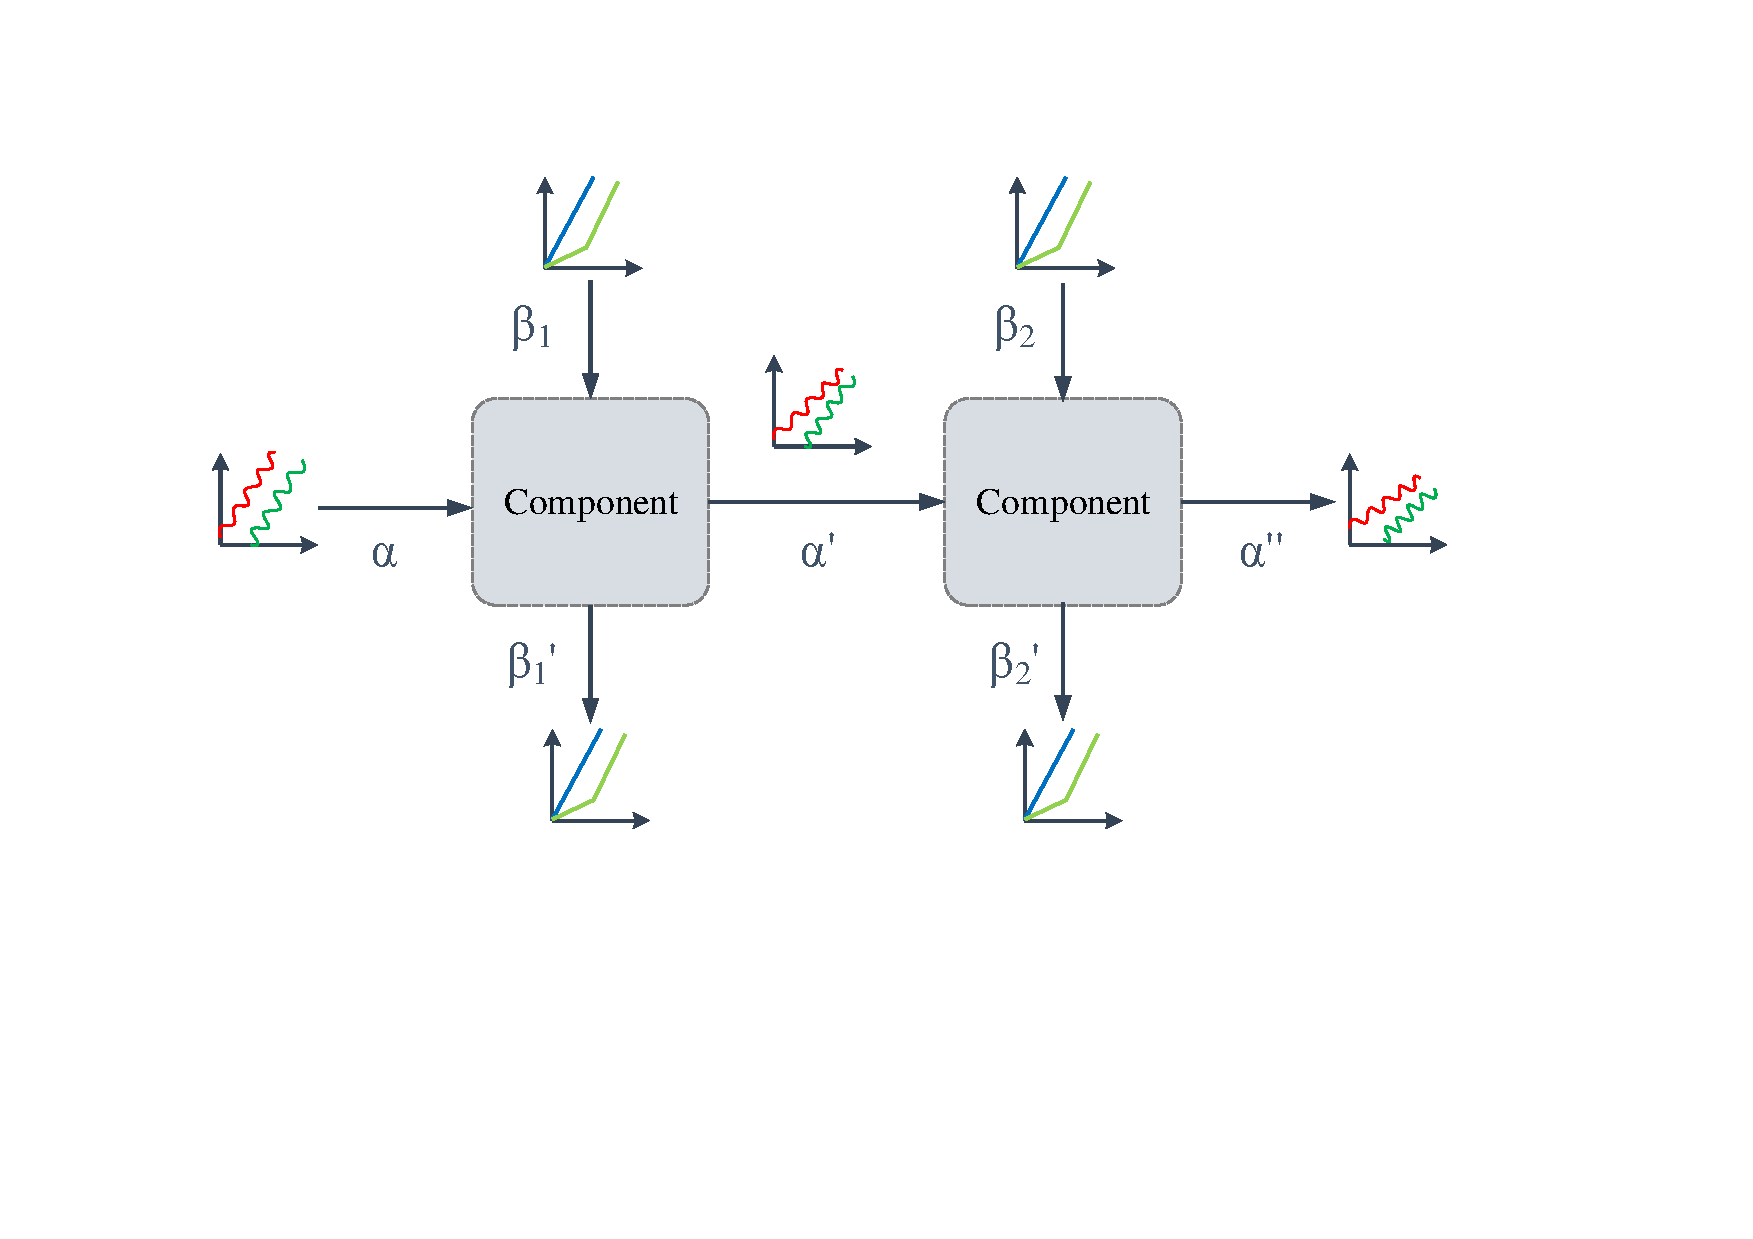
\includegraphics[scale=0.3]{figures/fig1}
\centering
\caption{A model consisting of two components.}
\label{fig1}
\end{figure}
\begin{figure}[H]
\centering
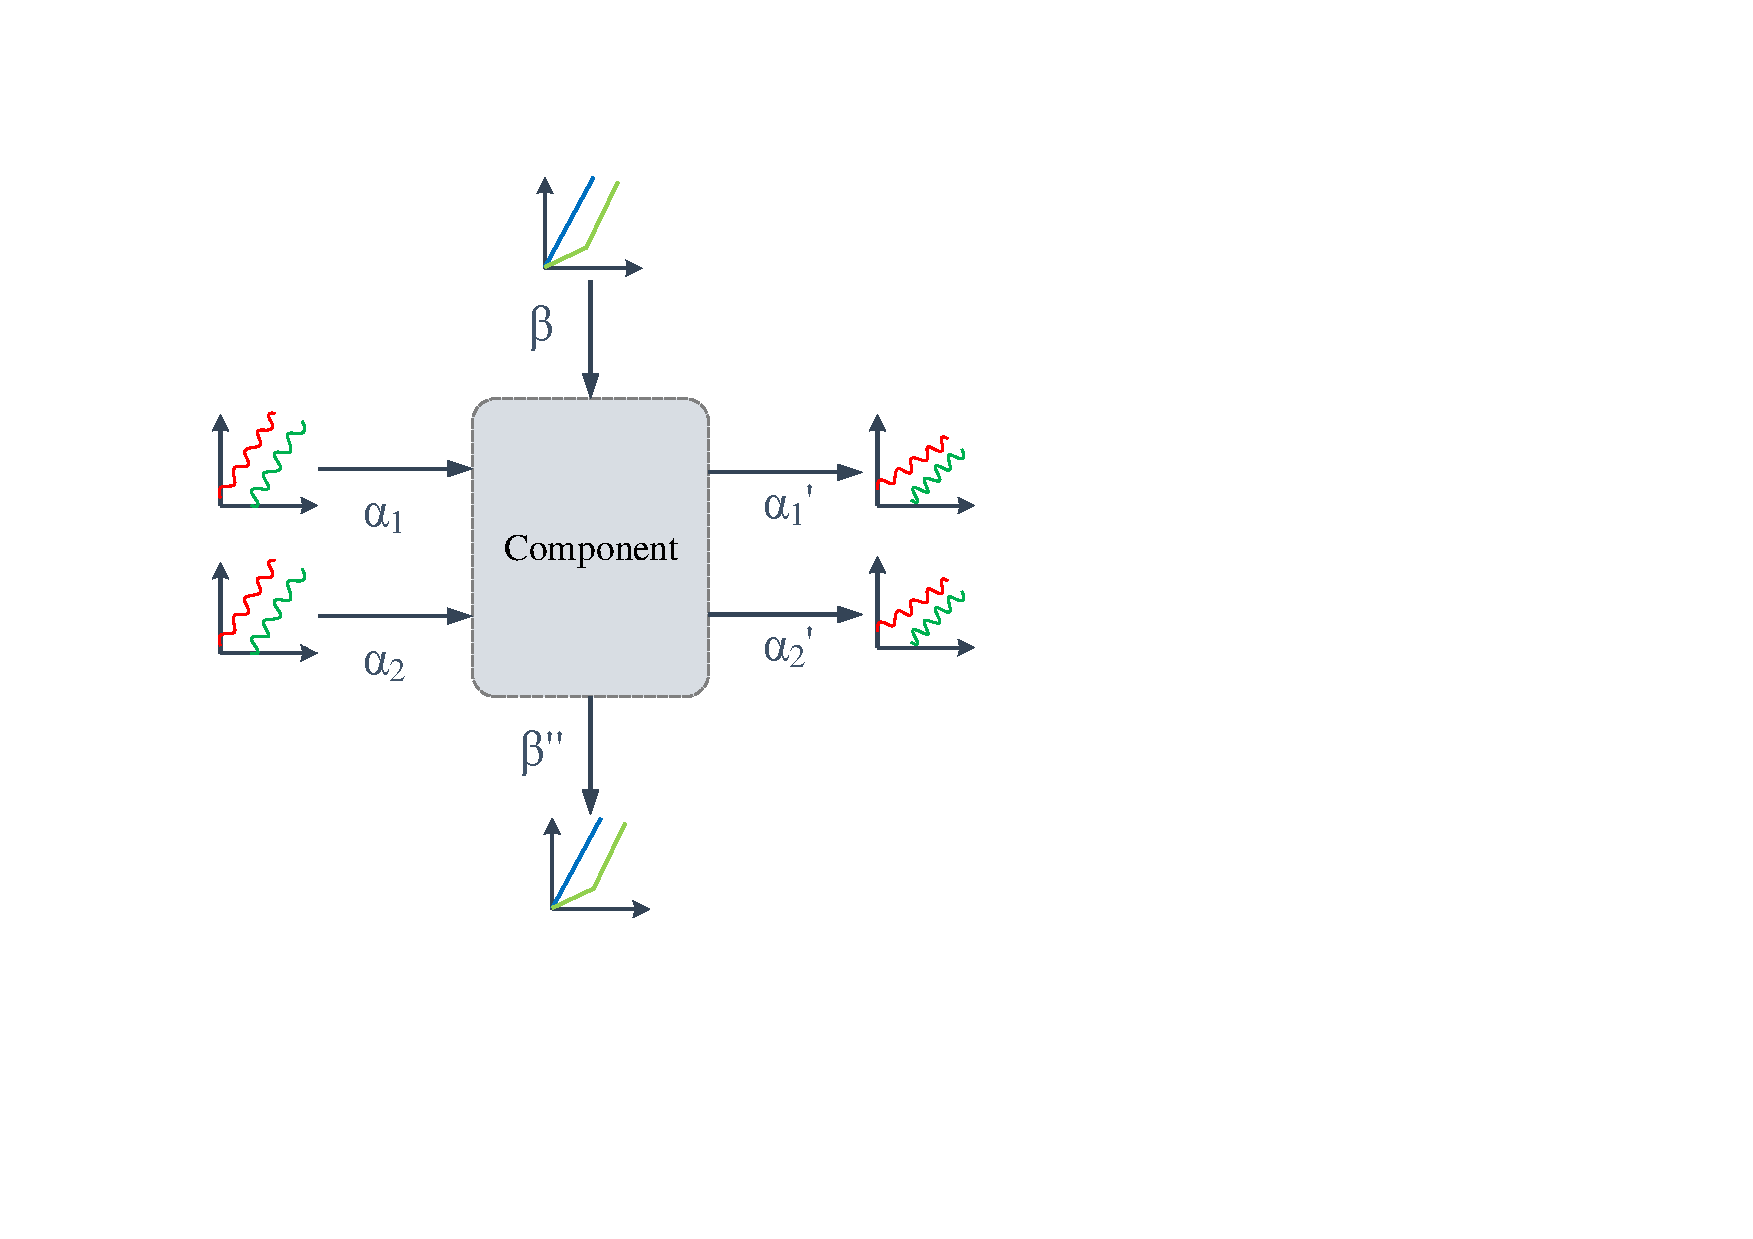
\includegraphics[scale=0.3]{figures/fig2}
\centering
\caption{A model consisting of two flows.}
\label{fig2}
\end{figure}

In the first case, we consider the impact of a single data flow through different components on the arrival curve.
As shown in {Figure} \ref{fig1}, suppose a TT flow constrained by arrival curve $\alpha$ passes through two components. After the first component processing, the outgoing arrival curve of data flow becomes $\alpha'$. The data flow continues to enter into the second component with its arrival curve $\alpha'$. Finally, an outgoing arrival curves $\alpha''$ is obtained.

In another combination, there are two different flows passing through the same component at the same time. The component provides services to process different flows in order of priority. As shown in {Figure} \ref{fig2}, the resource model will first serve the high-priority flow $\alpha_1$ with service curve $\beta$. Thereafter, the~remaining resource is used to process the low-priority flow $\alpha_2$. With $\alpha_1$ and $\alpha_2$ done, the remaining service curve is known as $\beta''$. These remaining resources might be used to process other lower priority flows. In~the worst case, the available resources are exhausted when processing $\alpha_1$, thereby preventing the remaining resources from satisfying $\alpha_2$, which in turn will block the low-priority flows until the next slot.

Based on a system architecture and the combination of the above two modes, an abstract model of the system can be constructed. The abstract model includes all the necessary information for network performance analysis for the next calculation.

%%%%%%%%%%%%%%%%%%%%%%%%%%%%%%%%%%%%%%%%%%
\section{Performance Analysis}
\label{analysis}

In the actual analysis network, it is easily to get the arrival curve of TT flows in the initial node according to TT period, size and other information. However, as flows are transmitted,  the arrival curve at each node gets changed with delay and jitter. Simultaneously, according to the transmission capacity, the service curve in each node can be obtained. But after processing incoming data flows, transmission resources are consumed, and the service curve changes accordingly. In this paper, we use RTC framework to analyze the change process of arrival curves and service curves. The analyzable performance metrics mainly include delay bounds, backlog bounds and resource utilization. In this section we formalize these notions and state the formulas for deriving these performance metrics.

Delay is an important performance characteristic in computer networks, which reflects to the time required for data flows to be transmitted from source to destination through the network.~Typically, network delay consists of processing, queuing, transmission and propagation delays.~{In this study, delay~mainly refers to processing and queuing delay. Suppose that transmission rate is determined; then~transmission delay can be calculated by the relative calculating formula.~Propagation delay is generally of the order of nanoseconds and negligible in the ideal situation.} Delay bound can be expressed by the following~inequality:
 \begin{equation}
   \begin{aligned}
   delay &\leq \sup_{t \ge 0} \{\inf\{\tau \ge 0:\alpha^u(t) \leq \beta^l(t+\tau)\}\}\\
   \end{aligned}
\end{equation}

Backlog is another performance metric, which is often related to the determination of worst-case buffer fill levels. When high volumes of traffic reach a processing node, if the resources are occupied, the~traffic first enters a buffer and waits for scheduling. Thus, the processing node needs to reserve a buffer space; that is, the maximum backlog needs to be considered. The backlog satisfies
\begin{equation}
   \begin{aligned}
&	backlog \leq \sup_{t \geq 0} \{\alpha^u(t)-\beta^l(t)\}\\
   \end{aligned}
\end{equation}


As depicted in {Figure} \ref{cur}, the maximum delay corresponds to the maximal horizontal distance between $\alpha^u$ and $\beta^l$, represented by $d_{max}$. The backlog is bounded by the vertical deviation between the arrival and service curves, signified by $b_{max}$.

\begin{figure}[H]
\centering
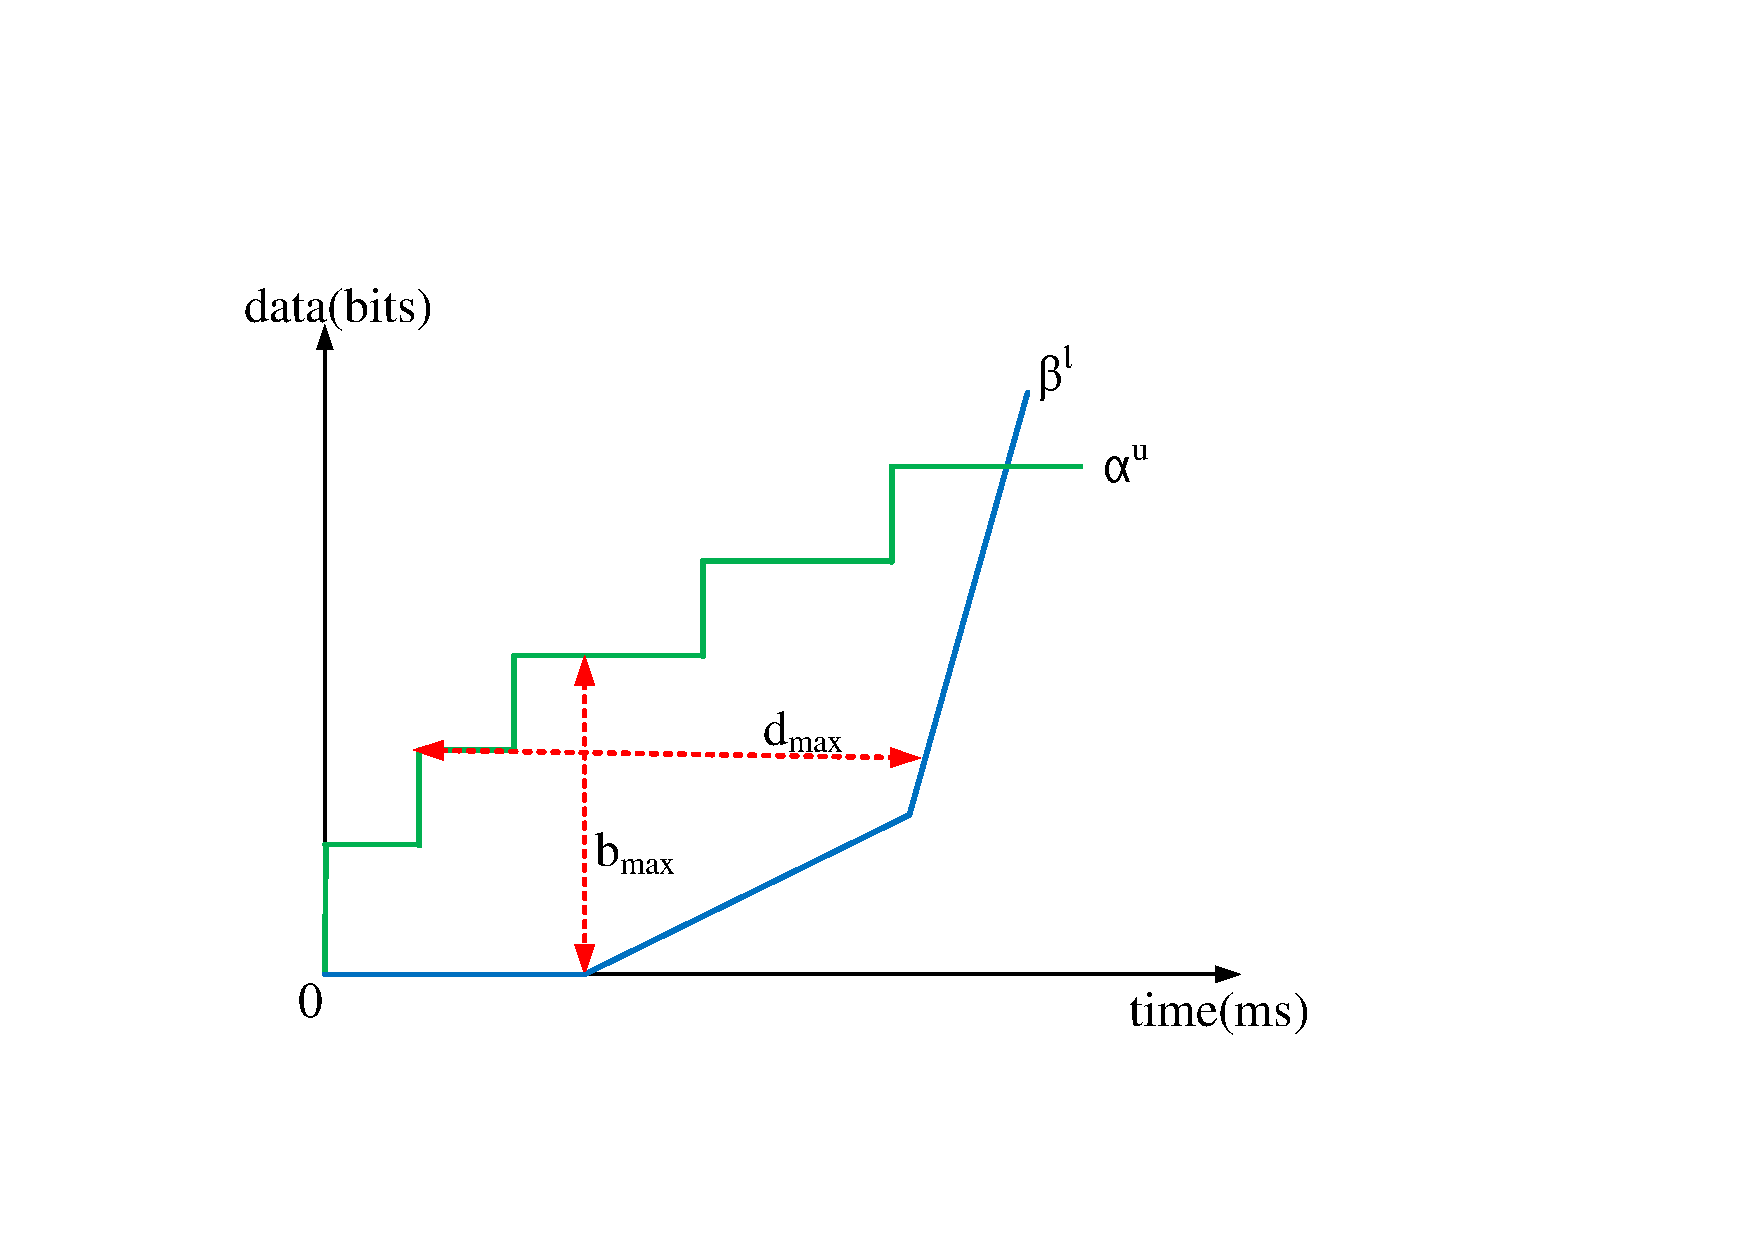
\includegraphics[scale=0.35]{figures/curve}
\caption{Abstract representation of delay and backlog.}
\label{cur}
\end{figure}
Finally, the resources of each node are limited in TTEthernet. The network system is needed to not only satisfy real-time and reliability requirements for critical traffic, but also improve resource utilization as far as possible.
Let $\beta^u$ and $\beta^{l'}$ be the initial upper service curve and the final lower (remaining) service curve of a resource; then its long term maximum utilization can be given by
\begin{gather}
\begin{aligned}
 	utilization = \lim_{\Delta \to \infty} \cfrac{\beta^u(\Delta)-\beta^{l'}(\Delta)}{\beta^u(\Delta)} %\label{con:23}
 \end{aligned}
\end{gather}

{Generally, non-critical traffic (such as BE) use the remaining bandwidth of the network. For critical traffic, the fewer resources that are overhead while barely impacting the delay, the more resources that can be utilized for non-critical traffic. Thus, resources exploited in an optimal way facilitate higher resource utilization of the whole network system.}

Through the calculation of delay bounds, backlog bounds and resource utilization, a comprehensive performance analysis {over} TTEthernet can be undertaken. Meanwhile, it also can be used to {evaluate} potential bottlenecks that exist in a {network system}.

%%%%%%%%%%%%%%%%%%%%%%%%%%%%%%%%%%%%%%%%%%
\section{Case Study}
\label{case}

In this section, a case study is demonstrated to evaluate the feasibility of the proposed performance analysis framework. The TTEthernet system has a topology of two TTE switches and six end systems, running six TT flows and eight RC flows in {Figure} \ref{ach}. The transmission rate of this network is 100 Mbps. The details of the TT and RC flows are presented in Table \ref{tab1}. The flow name, route, period (or BAG) and size are presented in columns 1, 2, 3 and 4, respectively. The scheduled time slots for each TT flow are displayed in Table \ref{tab2}.

\begin{figure}[H]
\centering
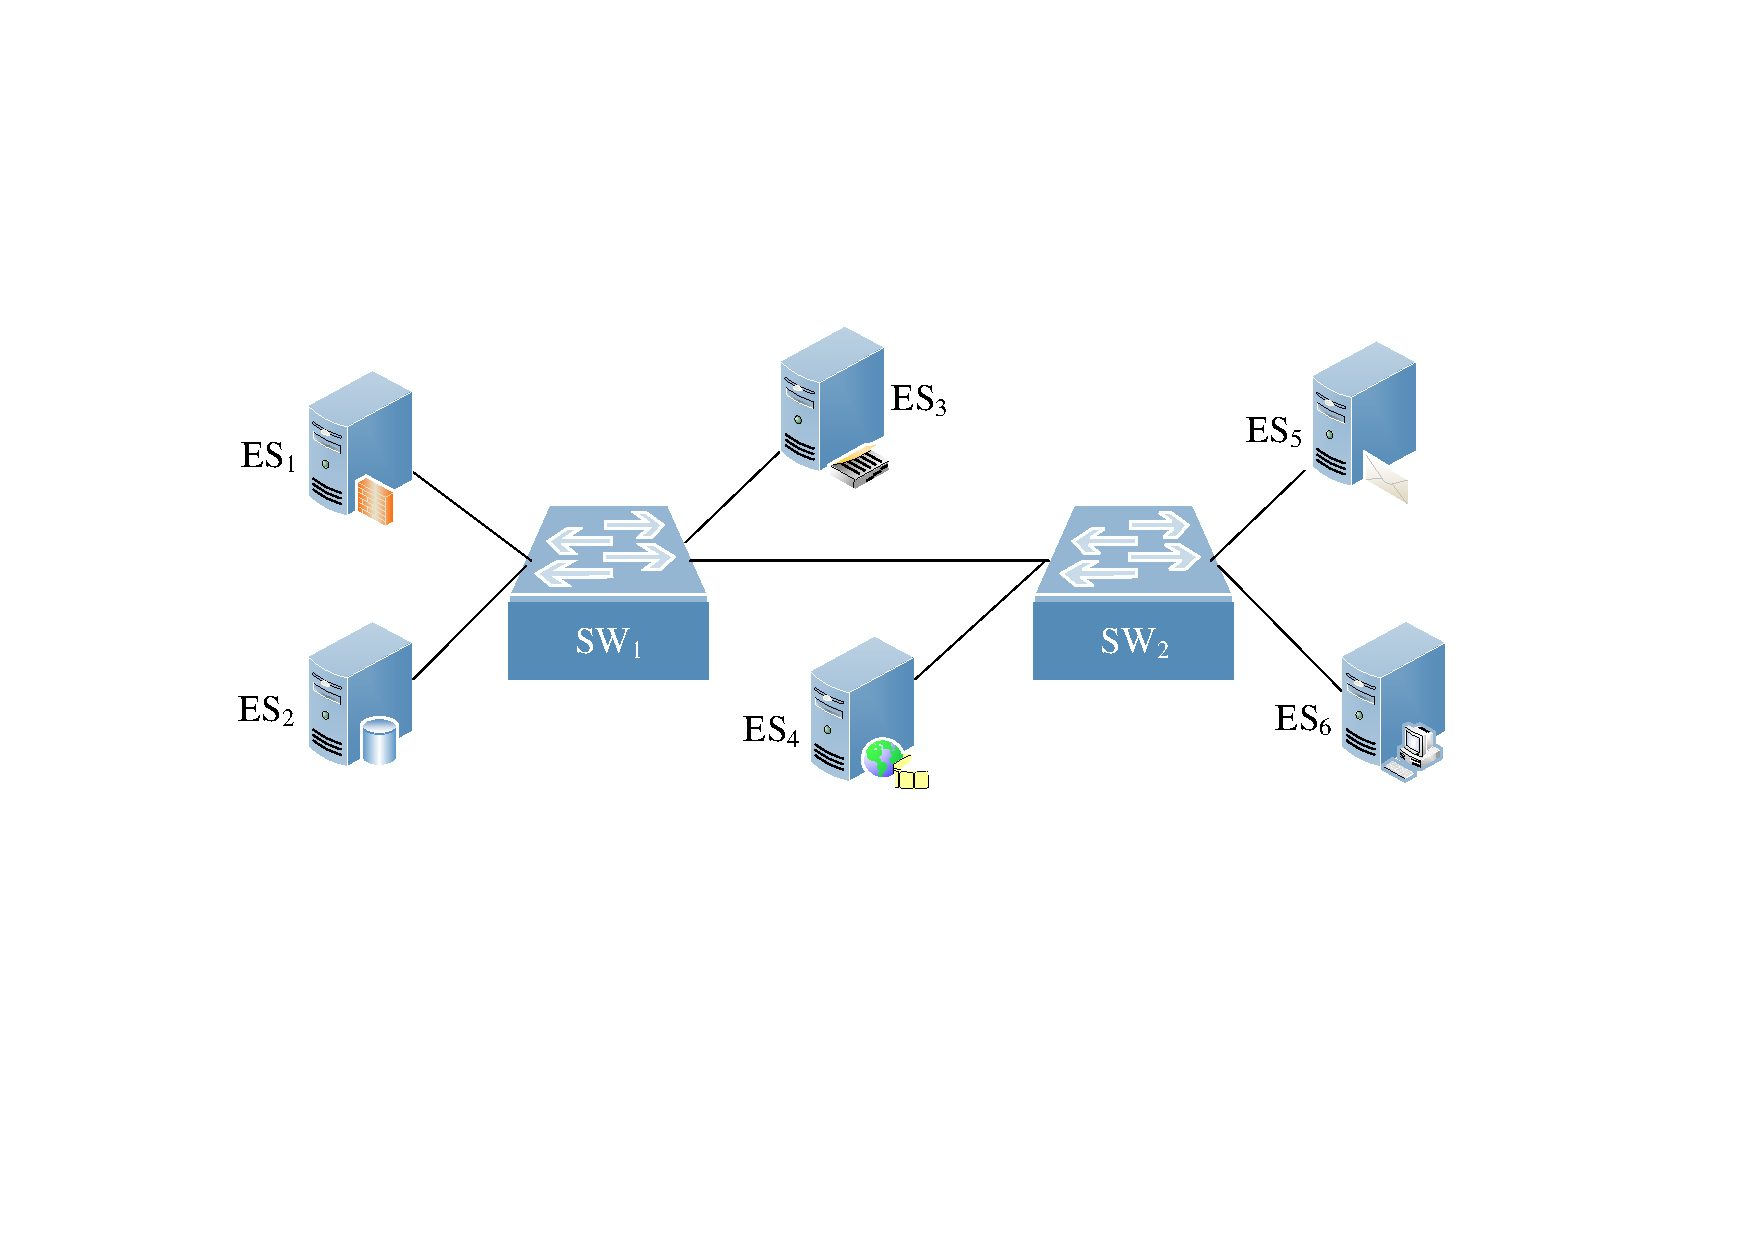
\includegraphics[width=0.6\textwidth]{figures/archi}
\caption{TTEthernet topology.}
\label{ach}
\end{figure}
\unskip



 \begin{table}[H]
            \centering
            \caption{The details of TT and RC flows.}\label{tab1}
            \begin{tabular}{ccm{1.7cm}<{\centering}m{1.3cm}<{\centering}}
\toprule
{\bf  Flow} & {\bf  Route} & {\bf   Period (ms)} & {\bf  Size (B)}\\
\midrule
$TT_1$ & $ES_1$-$SW_1$-$SW_2$-$ES_5$ & 2 & 880\\

$TT_2$ & $ES_1$-$SW_1$-$ES_3$ & 1 & 730\\

$TT_3$ & $ES_1$-$SW_1$-$SW_2$-$ES_6$ & 2 & 340\\

$TT_4$ & $ES_2$-$SW_1$-$SW_2$-$ES_6$ & 2 & 560 \\

$TT_5$ & $ES_2$-$SW_1$-$ES_3$ & 2 & 1300 \\

$TT_6$ & $ES_4$-$SW_2$-$ES_5$ & 2 & 900\\
\midrule
{\bf  Flow} & {\bf  Route} & {\bf  BAG (ms)} & {\bf  Size (B)}\\
\midrule
$RC_1$ & $ES_1$-$SW_1$-$SW_2$-$ES_6$ & 2 & 1320 \\

$RC_2$ & $ES_2$-$SW_1$-$SW_2$-$ES_5$ & 2 & 890\\

$RC_3$ & $ES_2$-$SW_1$-$ES_3$ & 4 & 1250\\

$RC_4$ & $ES_4$-$SW_2$-$ES_5$ & 2 & 760\\

$RC_5$ & $ ES_2$-$SW_1$-$SW_2$-$ES_6$ & 8 & 900\\

$RC_6$ & $ES_1$-$SW_1$-$SW_2$-$ES_5$ & 2 & 1050\\

$RC_7$ & $ES_1$-$SW_1$-$SW_2$-$ES_5$ & 2 & 1200\\

$RC_8$ & $ES_1$-$SW_1$-$ES_3$ & 2 & 980\\
\bottomrule
\end{tabular}
 \end{table}
\unskip
        \begin{table}[H]
         \centering
\caption{TT schedule.}
        \begin{tabular}{m{1.6cm}<{\centering}m{0.9cm}<{\centering}m{2.2cm}<{\centering}}

\toprule
{\bf  Link} & {\bf VL ID} & {\bf Time Slot (ms)}\\
\midrule
\multirow{3}{*}{[$ES_1$, $SW_1$]} & 1 & [0.65,0.90]\\

& 2 & [0.35,0.60] \\

& 3 & [1.05,1.30] \\
\midrule
\multirow{2}{*}{[$ES_2$, $SW_1$]} & 4 & [1.70,1.95] \\

& 5 & [1.05,1.30]\\
\midrule
\multirow{3}{*}{[$SW_1$, $SW_2$]} & 1 & [1.40,1.65]\\

& 3 & [0.10,0.35]\\

& 4 & [0.75,1.00]\\
\midrule
\multirow{2}{*}{[$SW_1$, $ES_3$]} & 2 & [0.45,0.70]\\

& 5 & [0.80,1.05]\\
\midrule

[$ES_4$, $SW_2$] & 6 & [1.35,1.60]\\

\midrule
\multirow{2}{*}{[$SW_2$, $ES_5$]} & 1 & [0.65,0.90]\\

& 6 & [1.00,1.25]\\
\midrule
\multirow{2}{*}{[$SW_2$, $ES_6$]} & 3 & [0.80,1.05]\\

& 4 & [1.70,1.95]\\
\bottomrule
\end{tabular}
\label{tab2}
 \end{table}


During nonsynchronous operations such as cold start and restart in TTE networks, end systems dispatch PCFs (such as CS frame and CA frame) to TTE switches. Then, TTE switches generate a new PCF  and dispatch it to all end systems. The nonsynchronous operation process has no effect on TT flows. During clock synchronization, end systems plan to dispatch IN frames in each integration cycle duration, which might impact on TT transmission. Each PCF frame is a fixed size of 64 bytes. In this case study, it~is assumed that six end systems respectively dispatch PCF frames to the TTE switch at the beginning of the integration cycle duration. {In this experiment, we adopt a pessimistic approach to calculate the delay under the impact of clock synchronization; that is, PCFs preempt TT traffic in the worst case scenario.}

In accordance to the previous analysis, the data model based on the period, rate and other relevant information can be built, so as to get the arrival curve of TT flows. The resource model for each TT flow is built according to the TT schedule, so as to get the service curve. After building the data model and resource model, an abstract model of the system is generated based on the component model and the TTEthernet architecture in {Figure} \ref{ach}. {In the next part, we mainly discuss the impacts of three types of traffic integration strategies.} Under the preemption and timely-block strategies, it is observed that RC flows have no effect on the transmission of TT flows. Therefore, the two strategies can be regarded as one case to~analyze.

The worst-case delay of TT traffic can be obtained by the maximum horizontal distance between the modeled arrival curve and the modeled service curve, and concrete results are shown in {Figure} \ref{delay}. In~contrast to the preemption/timely block and shuffling integration mode, it is not difficult to find that under the shuffling integration strategy, the worst-case delay is higher than that under the other two integration strategies. This is consistent with the previous observations that the transmission of RC flows affect the transmission of TT flows.

\begin{figure}[H]
\centering
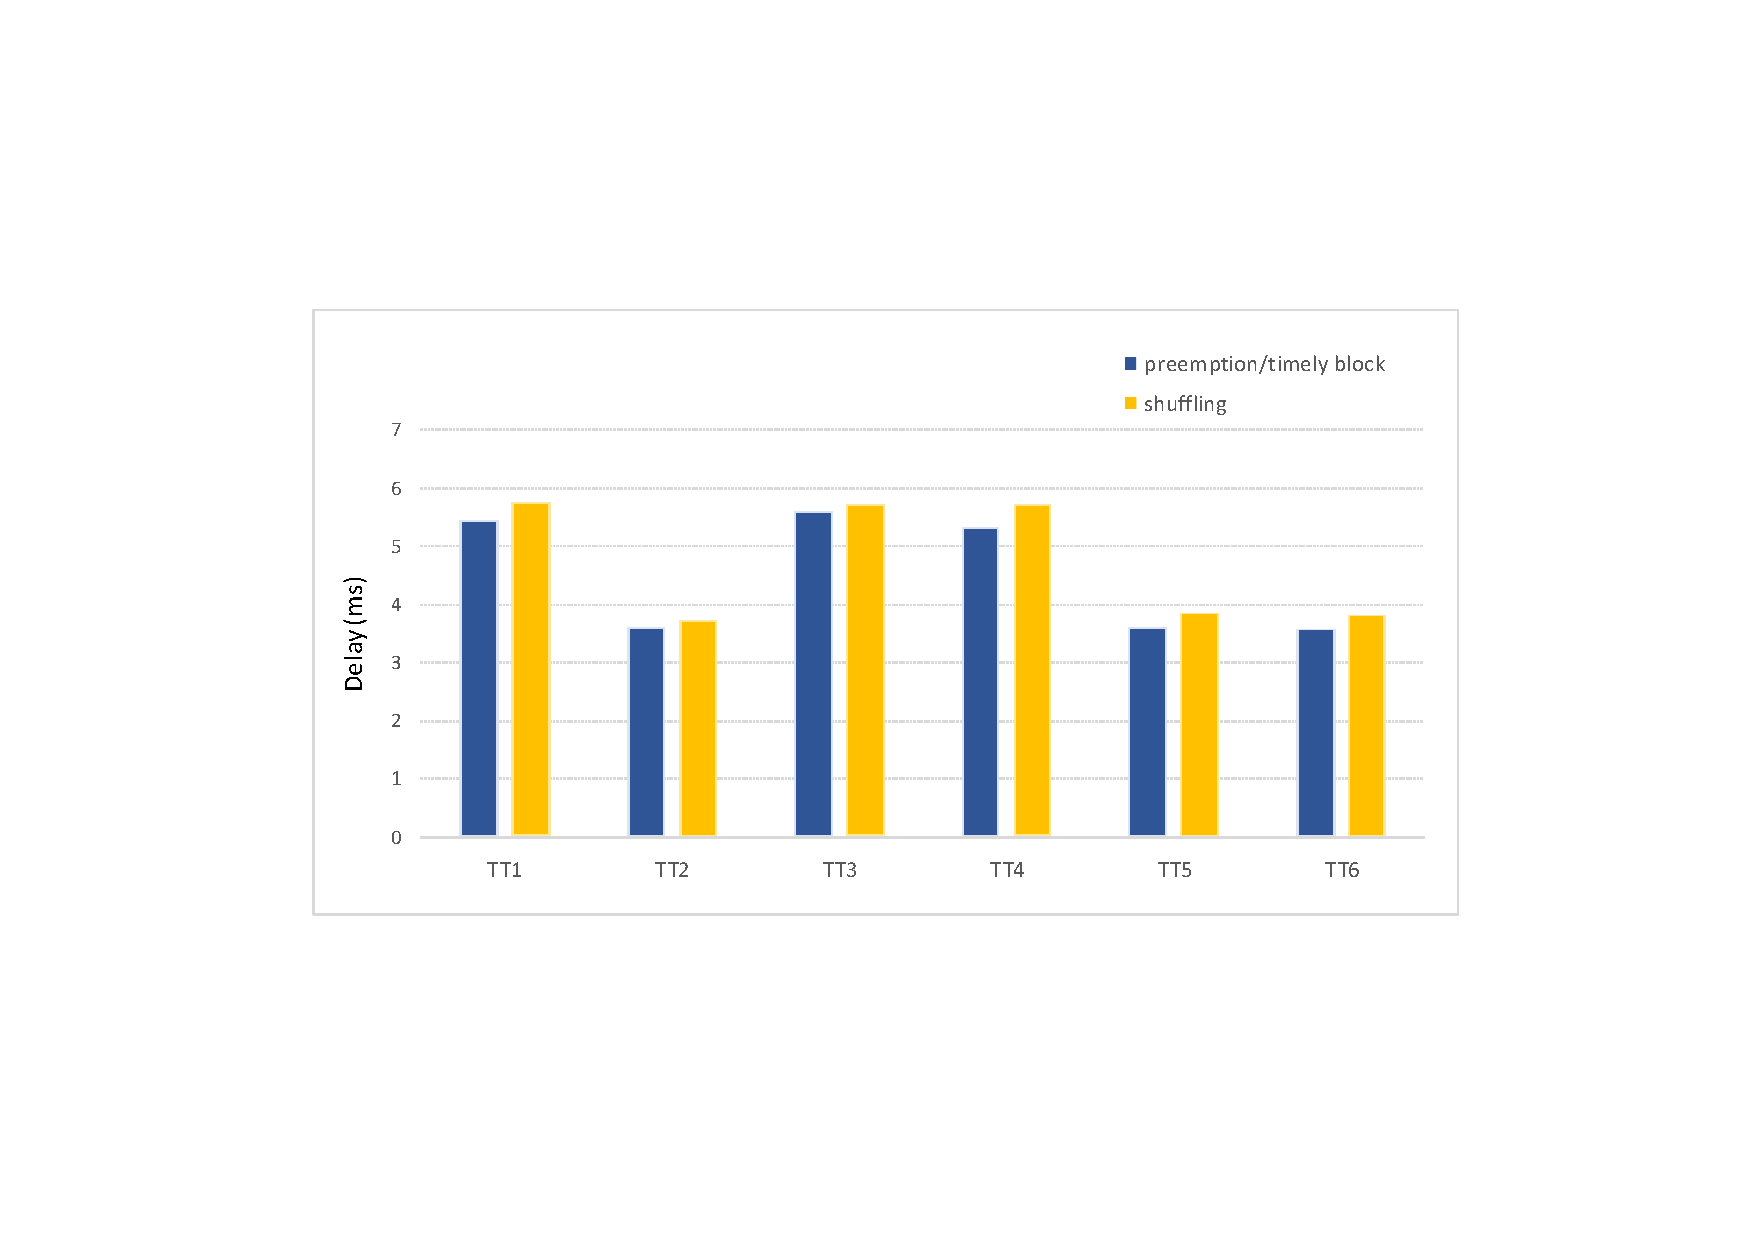
\includegraphics[width=0.65\textwidth]{figures/delay}
\caption{Worst-case delay under different traffic integration strategies.}
\label{delay}
\end{figure}

Through the previous analysis, it became evident that the worst-case backlog of processing node is the maximum vertical distance between the arrival curve and the service curve. Since the arrival curve in this case uses a staircase model, the influence of different integration strategies on the nodes can be ignored. The concrete buffer size in this case study is displayed in Table \ref{tab3}.

%\begin{table}[H]
%\caption{Worst-case backlog of processing node.}
%\centering
%%\small
%\begin{tabular}{cc}
%\toprule
%\textbf{Node}	& \textbf{WCB (bits)}\\
%\midrule
%$ES_1$ & 24160\\
%$ES_2$ & 14880\\
%$SW_1$ & 78080\\
%$SW_2$ & 65280\\
%$ES_4$ & 7200\\
%\bottomrule
%\end{tabular}
%\label{tab3}
%\end{table}

\begin{table}[H]
%\small
\centering
\caption{Worst-case backlog of processing node.}

\begin{tabular}{cc}
\toprule
%\hline
\textbf{Node} & \textbf{WCB (bits)}\\
\midrule
%\hline
$ES_1$ & 24,160\\
%\cdashline{1-2}[0.7pt/2pt]
$ES_2$ & 14,880\\
%\cdashline{1-2}[0.7pt/2pt]
$SW_1$ & 78,080\\
%\cdashline{1-2}[0.7pt/2pt]
$SW_2$ & 65,280\\
%\cdashline{1-2}[0.7pt/2pt]
$ES_4$ & 7200\\
\bottomrule
%\hline
\end{tabular}
\label{tab3}
\end{table}


Finally, we consider the resource utilization of each link. The resource utilization is obtained according to the upper service curve and the final lower (remaining) service curve of the link, and the calculation process is given by Equation (39).

In this case, we take the resource utilization on the ES1--SW1 link as an example to calculate the resource utilization of the transmission of TT1, TT2 and TT3 flows under three integration strategies, and~the results are shown in {Figure} \ref{util}. It can be observed that resource utilization under shuffling strategy is higher in comparison to the other two strategies.

\begin{figure}[H]
\centering
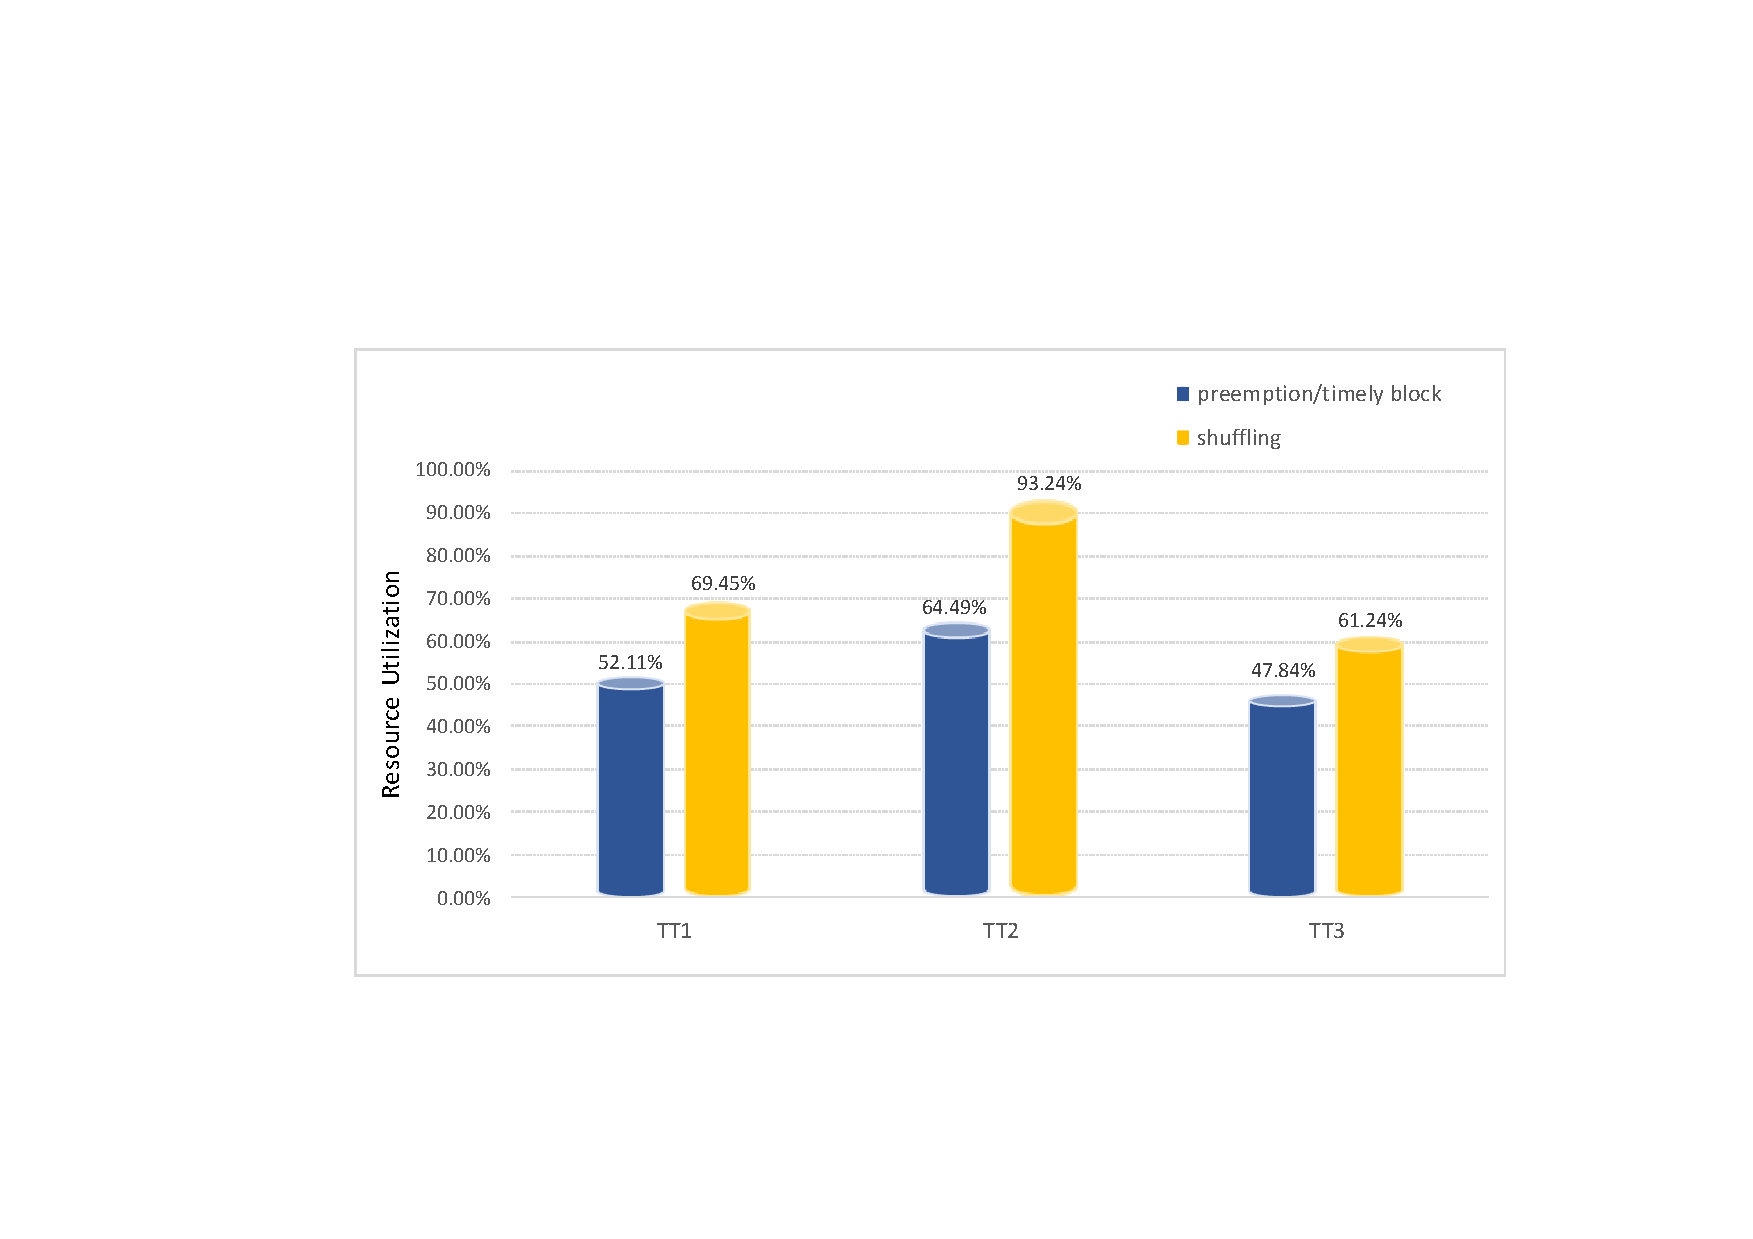
\includegraphics[width=0.6\textwidth]{figures/utilization}
\caption{Resource utilization under different traffic integration strategies.}
\label{util}
\end{figure}

In summary, under the preemption/timely block integration strategy, the worst-case delay of TT traffic is lower, and the system has higher real-time performance. Under the shuffling integration strategy, though the delay of TT flows increases slightly, the delay of RC flows can be guaranteed. From the aspect of resource utilization, the performance under the shuffling strategy gets better. Which integration strategy to choose should be combined with the real-time requirements of the system. The experimental results show that the proposed performance analysis framework is feasible in evaluating the performance of TTEthernet. Moreover, the analysis results can assist in selecting the appropriate scheduling algorithm and traffic integration strategy for the system.

%%%%%%%%%%%%%%%%%%%%%%%%%%%%%%%%%%%%%%%%%%
\section{Conclusions}
\label{con}
In this paper, we proposed a TTEthernet performance analysis framework, and conducted a feasibility analysis for the scheduling of critical traffic in the network. We presented the data model and resource model, and built the abstract model with system architecture and component mode. Then RTC was used to calculate the worst-case end-to-end delay of TT traffic in the network, the cache size of nodes and the utilization of network resources, so as to evaluate the performance of the system. During the modeling process, the~influences of clock synchronization and traffic integration strategies on the acceptance window for the critical traffic were analyzed to ensure the reliability of this study's results. Finally, the feasibility of this study's proposed performance analysis framework was verified through a specific case study. According to the experimental results, different integration strategies can be chosen for designing the network architecture which meets the different levels of real-time requirements. This is conducive to saving money and improving the utilization of system resources.

%%%%%%%%%%%%%%%%%%%%%%%%%%%%%%%%%%%%%%%%%%
%\section{Patents}
%This section is not mandatory, but may be added if there are patents resulting from the work reported in this manuscript.

%%%%%%%%%%%%%%%%%%%%%%%%%%%%%%%%%%%%%%%%%%
\vspace{6pt}

%%%%%%%%%%%%%%%%%%%%%%%%%%%%%%%%%%%%%%%%%%
%% optional
%\supplementary{The following are available online at \linksupplementary{s1}, Figure S1: title, Table S1: title, Video S1: title.}

% Only for the journal Methods and Protocols:
% If you wish to submit a video article, please do so with any other supplementary material.
% \supplementary{The following are available at \linksupplementary{s1}, Figure S1: title, Table S1: title, Video S1: title. A supporting video article is available at doi: link.}

%%%%%%%%%%%%%%%%%%%%%%%%%%%%%%%%%%%%%%%%%%
%\authorcontributions{For research articles with several authors, a short paragraph specifying their individual contributions must be provided. The following statements should be used ``Conceptualization, X.X. and Y.Y.; methodology, X.X.; software, X.X.; validation, X.X., Y.Y. and Z.Z.; formal analysis, X.X.; investigation, X.X.; resources, X.X.; data curation, X.X.; writing--original draft preparation, X.X.; writing--review and editing, X.X.; visualization, X.X.; supervision, X.X.; project administration, X.X.; funding acquisition, Y.Y. All authors have read and agreed to the published version of the manuscript.'', please turn to the  \href{http://img.mdpi.org/data/contributor-role-instruction.pdf}{CRediT taxonomy} for the term explanation. Authorship must be limited to those who have contributed substantially to the work reported.}

\authorcontributions{Conceptualization, Y.H. and J.S.; methodology, X.Y. and Z.C.; resources, J.S. and Y.H.; performance analysis, X.Y.; investigation, X.Y. and Z.C.; writing---original draft preparation, X.Y. and Z.C.; writing---review and editing, X.Y. and Y.H.; supervision, Y.H.; project administration, J.S. All authors have read and agreed to the published version of the manuscript.}
%%%%%%%%%%%%%%%%%%%%%%%%%%%%%%%%%%%%%%%%%%
\funding{This research is partially supported by Shanghai Municipal Ecnomic and Infomatization Commission Project (2018-GYHLW-02012), the Shanghai Science and Technology Committee Rising-Star Program (number 18QB1402000) and Science and Technology Commission of Shanghai Municipality Project (number 18ZR1411600).}

%%%%%%%%%%%%%%%%%%%%%%%%%%%%%%%%%%%%%%%%%%
%\acknowledgments{In this section you can acknowledge any support given which is not covered by the author contribution or funding sections. This may include administrative and technical support, or donations in kind (e.g., materials used for experiments).}

%%%%%%%%%%%%%%%%%%%%%%%%%%%%%%%%%%%%%%%%%%
\conflictsofinterest{The authors declare no conflict of interest.}

%%%%%%%%%%%%%%%%%%%%%%%%%%%%%%%%%%%%%%%%%%
%% optional
\abbreviations{The following abbreviations are used in this manuscript:\\

\noindent
\begin{tabular}{@{}ll}
TTEthernet & time-triggered Ethernet\\
RTC & real-time calculus\\
TT & time-triggered\\
ET & event-triggered\\
RC & rate-constrained\\
BE & best-effort\\
AFDX & Avionics Full-Duplex Switched Ethernet\\
BAG & bandwidth allocation gap\\
PCF & protocol control frames\\
CS & cold-start\\
CA & cold-start acknowledge\\
IN & integration

\end{tabular}}

%%%%%%%%%%%%%%%%%%%%%%%%%%%%%%%%%%%%%%%%%%
%% optional
%\appendixtitles{no} % Leave argument "no" if all appendix headings stay EMPTY (then no dot is printed after "Appendix A"). If the appendix sections contain a heading then change the argument to "yes".
%\appendix
%\section{}
%\unskip
%\subsection{}
%The appendix is an optional section that can contain details and data supplemental to the main text. For example, explanations of experimental details that would disrupt the flow of the main text, but nonetheless remain crucial to understanding and reproducing the research shown; figures of replicates for experiments of which representative data is shown in the main text can be added here if brief, or as Supplementary data. Mathematical proofs of results not central to the paper can be added as an appendix.
%
%\section{}
%All appendix sections must be cited in the main text. In the appendixes, Figures, Tables, etc. should be labeled starting with `A', e.g., Figure A1, Figure A2, etc.

%%%%%%%%%%%%%%%%%%%%%%%%%%%%%%%%%%%%%%%%%%
\reftitle{References}

% Please provide either the correct journal abbreviation (e.g. according to the “List of Title Word Abbreviations” http://www.issn.org/services/online-services/access-to-the-ltwa/) or the full name of the journal.
% Citations and References in Supplementary files are permitted provided that they also appear in the reference list here.

%=====================================
% References, variant A: external bibliography
%=====================================
%\externalbibliography{yes}
%\bibliography{your_external_BibTeX_file}

%=====================================
% References, variant B: internal bibliography
%=====================================

\begin{thebibliography}{999}
\providecommand{\natexlab}[1]{#1}

\bibitem[Steiner and Bauer(2009)]{steiner2009ttethernet}
\textls[-5]{Steiner, W.; Bauer, G.
\newblock TTEthernet: Time-triggered services for Ethernet networks.
\newblock In Proceedings of the  2009 IEEE/AIAA 28th Digital Avionics Systems Conference, Orlando, FL, USA, 23--29 October %MDPI: Newly added information, please confirm. ----------Confirmed.
 2009; pp.~1.B.4--1--1.B.4--1.}

\bibitem[Steiner \em{et~al.}(2018)Steiner, Bauer, Hall, and
  Paulitsch]{steiner2018time}
Steiner, W.; Bauer, G.; Hall, B.; Paulitsch, M.
\newblock Time-triggered ethernet. In \emph{Time-Triggered Communication;} CRC Press: Boca Raton, FL, USA, 2018; pp. 209--248.%----------Update.

\bibitem[Kopetz \em{et~al.}(2005)Kopetz, Ademaj, Grillinger, and
  Steinhammer]{kopetz2005time}
Kopetz, H.; Ademaj, A.; Grillinger, P.; Steinhammer, K.
\newblock The time-triggered ethernet (TTE) design.
\newblock  In Proceedings of the Eighth IEEE International Symposium on Object-Oriented Real-Time
  Distributed Computing (ISORC'05),  Seattle, WA, USA, 18--20 May 2005; pp. 22--33.%----------Confirmed.

\bibitem[Steiner \em{et~al.}(2009)Steiner, Bauer, Hall, Paulitsch, and
  Varadarajan]{TT}
Steiner, W.; Bauer, G.; Hall, B.; Paulitsch, M.; Varadarajan, S.
\newblock TTEthernet dataflow concept.
\newblock  In Proceedings of the 2009 Eighth IEEE International Symposium on Network Computing and
  Applications, Cambridge, MA, USA,  9--11 July 2009; pp. 319--322.%----------Confirmed.

\bibitem[Suethanuwong(2012)]{suethanuwong2012scheduling}
Suethanuwong, E.
\newblock Scheduling time-triggered traffic in TTEthernet systems.
\newblock  In Proceedings of 2012 IEEE 17th International Conference on Emerging
  Technologies \& Factory Automation (ETFA 2012), Krakow, Poland, 17--21 September 2012; pp. 1--4. %----------Confirmed.

\bibitem[Craciunas \em{et~al.}(2014)Craciunas, Oliver, and
  Ecker]{craciunas2014optimal}
Craciunas, S.S.; Oliver, R.S.; Ecker, V.
\newblock Optimal static scheduling of real-time tasks on distributed
  time-triggered networked systems.
\newblock  In Proceedings of the 2014 IEEE Emerging Technology and Factory
  Automation (ETFA),  Barcelona, Spain, 16--19 September 2014; pp. 1--8. %----------Confirmed.

\bibitem[Zhang \em{et~al.}(2018)Zhang, He, Lu, and Xiong]{zhang2018imporosity}
Zhang, Y.; He, F.; Lu, G.; Xiong, H.
\newblock An imporosity message scheduling based on modified genetic algorithm
  for time-triggered Ethernet.
\newblock {\em Sci. China Inf. Sci.} {\bf 2018}, {\em
  61},~019102.

\bibitem[Abuteir and Obermaisser(2015)]{abuteir2015scheduling}
Abuteir, M.; Obermaisser, R.
\newblock Scheduling of rate-constrained and time-triggered traffic in
  multi-cluster ttethernet systems.
\newblock  In Proceedings of the 2015 IEEE 13th International Conference on Industrial Informatics
  (INDIN),  Cambridge, UK, 22--24 July 2015; pp. 239--245. %----------Confirmed.

\bibitem[Zhao \em{et~al.}(2017)Zhao, Pop, Li, Chen, and Xiong]{zhao2017timing}
Zhao, L.; Pop, P.; Li, Q.; Chen, J.; Xiong, H.
\newblock Timing analysis of rate-constrained traffic in TTEthernet using
  network calculus.
\newblock {\em Real-Time Syst.} {\bf 2017}, {\em 53},~254--287.

\bibitem[Chakraborty \em{et~al.}(2003)Chakraborty, K{\"u}nzli, and
  Thiele]{chakraborty2003general}
Chakraborty, S.; K{\"u}nzli, S.; Thiele, L.
\newblock A General Framework for Analysing System Properties in Platform-Based
  Embedded System Designs.
\newblock In  Proceedings of the conference on Design, Automation and Test in
  Europe, Munich, Germany, 7 March 2003; Volume~3, pp. 10190--10195. %----------Confirmed.

\bibitem[Zhang \em{et~al.}(2019)Zhang, Liu, Shi, Huang, and
  Zhao]{zhang2019feasibility}
Zhang, P.; Liu, Y.; Shi, J.; Huang, Y.; Zhao, Y.
\newblock A Feasibility Analysis Framework of Time-Sensitive Networking Using
  Real-Time Calculus.
\newblock {\em IEEE Access} {\bf 2019}, {\em 7},~90069--90081.

\bibitem[Gavrilu{\c{t}} and Pop(2016)]{gavriluct2016traffic}
Gavrilu{\c{t}}, V.; Pop, P.
\newblock Traffic class assignment for mixed-criticality frames in TTEthernet.
\newblock {\em ACM Sigbed Rev.} {\bf 2016}, {\em 13},~31--36.

\bibitem[Steiner and Dutertre(2011)]{steiner2011automated}
Steiner, W.; Dutertre, B.
\newblock Automated formal verification of the TTEthernet synchronization
  quality.
\newblock  In  Proceedings of the NASA Formal Methods Symposium, Pasadena, CA, USA, 18--20 April 2011; Springer:  Berlin, Germany, 2011; pp. 375--390. %----------Confirmed.

\bibitem[Tamas-Selicean \em{et~al.}(2012)Tamas-Selicean, Pop, and
  Steiner]{tamas2012synthesis}
Tamas-Selicean, D.; Pop, P.; Steiner, W.
\newblock Synthesis of communication schedules for TTEthernet-based
  mixed- criticality systems.
\newblock   In Proceedings of the eighth IEEE/ACM/IFIP International Conference on
  Hardware/ Software Codesign and System Synthesis, Tampere, Finland, 7--12 October 2012; pp. 473--482.%MDPI: please add conference loaction and date. ----------Done.

\bibitem[Finzi and Craciunas(2019)]{finzi2019integration}
Finzi, A.; Craciunas, S.S.
\newblock Integration of SMT-based scheduling with RC network calculus analysis
  in TTEthernet networks.
\newblock  In Proceedings of the 2019 24th IEEE International Conference on Emerging Technologies and
  Factory Automation (ETFA), Zaragoza, Spain, 10--13 September 2019; pp. 192--199. %----------Confirmed.

\bibitem[Kermia(2017)]{kermia2017schedulability}
Kermia, O.
\newblock Schedulability analysis and efficient scheduling of rate constrained
  messages in the ttethernet protocol.
\newblock {\em Softw. Pract. Exp.} {\bf 2017}, {\em
  47},~1485--1499.

\bibitem[Thiele \em{et~al.}(2000)Thiele, Chakraborty, and
  Naedele]{thiele2000real}
Thiele, L.; Chakraborty, S.; Naedele, M.
\newblock Real-time calculus for scheduling hard real-time systems.
\newblock  In Proceedings of the 2000 IEEE International Symposium on Circuits and Systems (ISCAS), Geneva, Switzerland,  28--31 May 2000; Volume~4, pp. 101--104. %----------Confirmed.

\bibitem[Le~Boudec and Thiran(2001)]{le2001network}
Le~Boudec, J.Y.; Thiran, P.
\newblock {\em Network Calculus: A theory of Deterministic Queuing Systems for
  the Internet};  Springer Science \& Business Media:  Berlin, Germany, 2001; Volume 2050. %----------Confirmed.

\bibitem[Le~Boudec(1998)]{le1998application}
Le~Boudec, J.Y.
\newblock Application of network calculus to guaranteed service networks.
\newblock {\em IEEE Trans. Inf. Theory} {\bf 1998}, {\em
  44},~1087--1096.

\bibitem[Moy and Altisen(2010)]{moy2010arrival}
Moy, M.; Altisen, K.
\newblock Arrival curves for real-time calculus: The causality problem and its
  solutions.
\newblock  In Proceedings of the International Conference on Tools and Algorithms for the
  Construction and Analysis of Systems, Paphos, Cyprus, 20--29 March 2010; Springer: Berlin, Germany, 2010; pp. 358--372. %----------Confirmed.

\bibitem[Perathoner \em{et~al.}(2007)Perathoner, Wandeler, Thiele, Hamann,
  Schliecker, Henia, Racu, Ernst, and Harbour]{perathoner2007influence}
Perathoner, S.; Wandeler, E.; Thiele, L.; Hamann, A.; Schliecker, S.; Henia,
  R.; Racu, R.; Ernst, R.; Harbour, M.G.
\newblock Influence of different system abstractions on the performance
  analysis of distributed real-time systems.
\newblock  In~Proceedings of the 7th ACM \& IEEE International Conference on
  Embedded Software, Salzburg, Austria, 30 September--3 October  2007; pp. 193--202. %----------Confirmed.

\end{thebibliography}

%\begin{thebibliography}{999}
%% Reference 1
%\bibitem[Author1(year)]{ref-journal}
%Author1, T. The title of the cited article. {\em Journal Abbreviation} {\bf 2008}, {\em 10}, 142--149.
%% Reference 2
%\bibitem[Author2(year)]{ref-book}
%Author2, L. The title of the cited contribution. In {\em The Book Title}; Editor1, F., Editor2, A., Eds.; Publishing House: City, Country, 2007; pp. 32--58.
%\end{thebibliography}

% The following MDPI journals use author-date citation: Arts, Econometrics, Economies, Genealogy, Humanities, IJFS, JRFM, Laws, Religions, Risks, Social Sciences. For those journals, please follow the formatting guidelines on http://www.mdpi.com/authors/references
% To cite two works by the same author: \citeauthor{ref-journal-1a} (\citeyear{ref-journal-1a}, \citeyear{ref-journal-1b}). This produces: Whittaker (1967, 1975)
% To cite two works by the same author with specific pages: \citeauthor{ref-journal-3a} (\citeyear{ref-journal-3a}, p. 328; \citeyear{ref-journal-3b}, p.475). This produces: Wong (1999, p. 328; 2000, p. 475)


%%%%%%%%%%%%%%%%%%%%%%%%%%%%%%%%%%%%%%%%%%
%% optional
%\sampleavailability{Samples of the compounds ...... are available from the authors.}

%% for journal Sci
%\reviewreports{\\
%Reviewer 1 comments and authors’ response\\
%Reviewer 2 comments and authors’ response\\
%Reviewer 3 comments and authors’ response
%}

%%%%%%%%%%%%%%%%%%%%%%%%%%%%%%%%%%%%%%%%%%
\end{document}

